\chapter{Implementation}\label{chap:implementation}

\section{Work plan -- Work packages, deliverables}

\begin{todo}{}\color{red}
  Please provide the following:

  * brief presentation of the overall structure of the work plan;
  
  * timing of the different work packages and their components (Gantt chart or similar);

  * detailed work description, i.e.:
  
        - a list of work packages (table 3.1a);

        - a description of each work package (table 3.1b);

        - a list of major deliverables (table 3.1c);

  * graphical presentation of the components showing how they inter-relate (Pert chart or similar).

  Give full details. Base your account on the logical structure of the project and the stages in which it is to be carried out. The number of work packages should be proportionate to the scale and complexity of the project.

  You should give enough detail in each work package to justify the proposed resources to be allocated and also quantified information so that progress can be monitored, including by the Commission.

  Resources assigned to work packages should be in line with their objectives and deliverables. Note that the primary deliverables of Integrating Activities are access provision, optimised use, and further improvement of the services offered by the participating research infrastructures. You are advised to include a distinct work package on ‘management’ (see section 3.2) and on innovation, to indicate in the work package title the type of activity (Networking: NA, trans-national or virtual access: TA or VA, Joint Research: JRA) for non-management work packages (see Part D of the section “Specific features for Research Infrastructures” in the 2018-2020 Research Infrastructures Work Programme), and to give due visibility in the work plan to ‘dissemination and exploitation’ and ‘communication activities’, either with distinct tasks or distinct work packages.

  You will be required to include an updated (or confirmed) ‘plan for the dissemination and exploitation of results’ in both the periodic and final reports. This should include a record of activities related to dissemination and exploitation that have been undertaken and those still planned. In the case of Integrating Activities this should moreover include dissemination of access opportunities and of the resulting use of the research infrastructure, as well as measures to assess or improve the innovation potential of the infrastructure. A report of completed and planned communication activities will also be required.

  {\bf Definitions:}

  - \underline{Work package}: means a major sub-division of the proposed project.

  - \underline{Deliverable}: means a distinct output of the project, meaningful in terms of the project's overall objectives and constituted by a report, a document, a technical diagram, a software etc.
\end{todo}

\begin{center}
\begin{tabular}{|c|c|c|c|c|c|c|c|}
\hline
    & 1 & 4 & 3 & 9 & 7 & 2 & 5 \\
\hline
\textsl{Inr} &   &   &   & x &   & x & x \\
\hline
\textsl{Str} &   &   & x &   &   &   &   \\
\hline
\textsl{Tou} & x &   &   &   &   &   &   \\
\hline
\textsl{Inn} &   & x &   &   & x & x &   \\
\hline
\textsl{Lie} &   & x &   &   &   &   &   \\
\hline
\textsl{Bol} & x &   &   &   &   &   &   \\
\hline
\textsl{Pra} &   & x &   &   &   &   & x \\
\hline
\textsl{Bel} &   &   & x &   &   &   & x \\
\hline
\textsl{Tum} & x &   & x &   &   &   &   \\
\hline
\textsl{Del} & x &   &   &   &   &   &   \\
\hline
\textsl{Sac} &   & x &   &   & x &   &   \\
\hline
\textsl{Fau} &   &   &   &   & x &   &   \\
\hline
\textsl{Lee} &   &   &   &   &   & x & x \\
\hline
\textsl{Sou} & x &   &   &   &   &   &   \\
\hline
\textsl{Got} & x &   &   &   &   &   &   \\
\hline
\textsl{Cha} & x &   & x &   &   &   &   \\
\hline
\textsl{Lmu} &   &   &   &   &   & x &   \\
\hline
\textsl{Imt} & x &   &   &   &   &   &   \\
\hline
\textsl{Bia} &   &   &   &   &   & x &   \\
\hline
\textsl{Dus} & x &   &   &   &   &   &   \\
\hline
\textsl{Oca} &   &   &   & x &   &   &   \\
\hline
\textsl{Cle} & x & x &   &   &   &   &   \\
\hline
\textsl{Bir} &   &   &   &   &   & x &   \\
\hline
\textsl{Cea} &   & x &   &   &   &   &   \\
\hline
\textsl{Stu} &   & x &   &   &   &   &   \\
\hline
\textsl{Irt} &   &   &   & x &   &   &   \\
\hline
\textsl{Edu} &   &   &   & x &   &   &   \\
\hline
\textsl{Pro} & x &   &   &   &   &   &   \\
\hline
\end{tabular}
\end{center}

\subsection*{Overall structure of the work plan}

Our work plan is divided into seven scientific work packages.  The
first group of work packages is dedicated to the networking activities
that are needed to gather the proofs today located in different
libraries.  The second to making these proofs accessible, beyond
trans-national and virtual access.  The third to joint research
activities that prepare the future of Logipedia.

Together with these seven scientific work packages, two more work
packages are dedicated to dissemination, communication and
exploitation and to management.

\begin{longtable}{|p{0.05\textwidth}|p{0.15\textwidth}|p{0.17\textwidth}|p{0.55\textwidth}|}
\hline
\rowcolor{color2}\multicolumn{4}{|l|}{\bf Networking activities:}\\
\hline
WP1
&
Integration &
Jesper Cockx

(Delft)
&
Instrument the systems for which we already know how to encode the
proofs in Dedukti, and make these proofs available in Logipedia.
\\
\hline
WP2
&
Automatic theorem proving
&
Chantal Keller

(Saclay)
& 
Develop automatic theorem provers to populate,
help, and benefit from Logipedia.
\\
\hline
WP3
&
Large libraries
&
Tobias Nipkow

(M\"unchen)
&
Export large dedicated libraries in curated form 
to Logipedia for end-user applications.
\\
\hline
\end{longtable}

\begin{longtable}{|p{0.05\textwidth}|p{0.15\textwidth}|p{0.17\textwidth}|p{0.55\textwidth}|}
\hline
\rowcolor{color2}\multicolumn{4}{|l|}{\bf Trans-national and virtual access:}\\
\hline
WP4
&
Access
&
Frédéric Blanqui

(Inria)
&
Define and build the Logipedia hardware and software infrastructure in
which the proofs will be integrated.
\\
\hline
WP5
&
Structure of the encyclopedia
&
Florian Rabe

(Erlangen)
&
Provide infrastructure for the structured ontological representation
of libraries and use it to enrich the information about formal
libraries in Logipedia.
\\
\hline
\end{longtable}


\begin{longtable}{|p{0.05\textwidth}|p{0.15\textwidth}|p{0.17\textwidth}|p{0.55\textwidth}|}
\hline
\rowcolor{color2}\multicolumn{4}{|l|}{\bf Joint research activities:}\\
\hline
WP6
&
Theories
&
Cezary Kaliszyk

(Inssbruck)
&
Bringing proof systems implementing a theory 
that has not yet been expressed in Dedukti to LIL 2 or better.
\\
\hline
WP7
&
Proof engineering
&
Filip Marić

(Belgrade)
&
Investigate methods for detecting concept alignments and apply
them to build a library of alignments present across the Logipedia database.
\\
\hline
\end{longtable}

\begin{longtable}{|p{0.05\textwidth}|p{0.15\textwidth}|p{0.17\textwidth}|p{0.55\textwidth}|}
\hline
\rowcolor{color2}\multicolumn{4}{|l|}{\bf Dissemination, communication, exploitation, and management:}\\
\hline
WP8
&
Dissemination, communication, and exploitation
&
Pascal Fontaine

(Liège)
&
Expand the use of Logipedia in research, industry, education, and publishing.
\\
\hline
WP9
&
Management
&
Gilles Dowek

(Inria)
&
Coordinate this large community, in a benevolent atmosphere, for optimal
efficiency.
\\
\hline
\end{longtable}

These work packages are diverse in the number of tasks and
partners. Some of them are large, while others are smaller. This
reflects the diversity of their natures and goals. The work package
``access'' for instance has a very definite and critical goal, it must
have a small number of partners and be focused on its goal. In
contrast, the work package ``theories'' requires experts in many
different systems.  It therefore has a larger number of partners.

{\color{red} Read objectives of WP: they must be objectives}



\subsection*{Detailed work description}

\begin{workplan}

% the template says: "indicate in the work package title the type of activity"

  \newcommand\na{(Networking activity)}
  \newcommand\tnva{(Trans-national and virtual access)}
  \newcommand\jra{(Joint research activity)}
  \newcommand\titlewp[3]{\bigskip\noindent\colorbox{color3}{\begin{minipage}\textwidth\bf Work Package #1: #2\end{minipage}}\input{workpackages/#3}}

\titlewp{1}{Integration \na}{instrumentation}

\titlewp{2}{Automatic theorem provers \na}{atpetc}

\titlewp{3}{Large libraries \na}{libraries}

\titlewp{4}{Accesses to the encyclopedia \tnva}{access}

\titlewp{5}{Structure of the encyclopedia \tnva}{structuring}

\titlewp{6}{Theories \jra}{theories}

\titlewp{7}{Proof engineering \jra}{alignment}

\titlewp{8}{Dissemination, communication and exploitation}{dissemination}

\titlewp{9}{Management}{management}

\end{workplan}

\subsubsection*{List of all deliverables}\label{sec:deliverables}

Here is an overview of the deliverables 
of the work packages. 

%In the table below, \emph{integrating work deliverables} (see top of
%section~\ref{sec:wplist}) are printed in boldface to mark them. They integrate
%contributions from multiple work packages.

{\footnotesize\inputdelivs{8cm}}

%%% Local Variables: 
%%% mode: latex
%%% TeX-master: "propB"
%%% End: 


\subsection*{Timing of the different work packages and their components}

\makeatletter
\newcounter{month}
\setcounter{month}{0}\@whilenum\value{month}<\numexpr\pdataref@aux{prop}{gen}{months}+1\do{\expandafter\newlength\csname offset\the\value{month}\endcsname\stepcounter{month}}
\def\offset@reset#1{\setcounter{month}{0}\@whilenum\value{month}<\numexpr\pdataref@aux{prop}{gen}{months}+1\do{\expandafter\setlength\csname offset\the\value{month}\endcsname{#1}\stepcounter{month}}}
\def\offset@incr#1#2{\expandafter\addtolength\csname offset#1\endcsname{#2}}
\def\offset@get#1{\expandafter\the\csname offset#1\endcsname}

\begin{ganttchart}
[
vgrid=true,
hgrid=true,
title height=1,
y unit title=\baselineskip,
y unit chart=.6\baselineskip,
x unit=10pt,
group peaks width=0,
group peaks height=0,
group left shift=0,
group right shift=0,
group top shift=.25,
group height=.5,
group/.append style={fill=blue},
group label node/.append style={font=\bf},
bar top shift=.25,
bar height=.5,
bar/.append style={fill=green,rounded corners=3pt,draw opacity=0},
bar label node/.append style={font=\footnotesize},
milestone left shift=.5,
milestone right shift=.5,
milestone top shift=0,
milestone height=1,
milestone/.append style={fill=yellow},
milestone inline label node/.append style={font=\scriptsize},
vrule/.style={very thick,red},
]
{1}{\pdataref@aux{prop}{gen}{months}}
\pgfdeclarelayer{delivs}
\pgfdeclarelayer{miles}
\pgfsetlayers{background,main,miles,delivs}
\gantttitle{\makebox[0pt][r]{\textbf{\textit{Month\ }}}}{0}
\gantttitlelist[title label node/.append style={font=\scriptsize}]{1,...,\pdataref@aux{prop}{gen}{months}}{1}
\edef\@wps{\pdataref@aux{all}{wp}{ids}}
\@for\@wp:=\@wps\do{
\\\\
\ganttgroup{\pdataRef{wp}{\@wp}{label}}{\pdataref@num{wp}{\@wp}{start}}{\pdataref@num{wp}{\@wp}{end}}
\begin{pgfonlayer}{delivs}
\offset@reset{.5pt}
\edef\@delivs{\pdataref@aux{\@wp}{delivs}{ids}}
\@for\@deliv:=\@delivs\do{
\ifodd\pdataref@num{deliv}{\@deliv}{due}
\ganttmilestone[inline,milestone inline label node/.append style={above right=0pt and -15pt}]{\pdataRef{deliv}{\@deliv}{label}}{\pdataref@num{deliv}{\@deliv}{due}}
\else
\ganttmilestone[inline,milestone inline label node/.append style={below right=\offset@get{\pdataref@num{deliv}{\@deliv}{due}} and -15pt}]{\pdataRef{deliv}{\@deliv}{label}}{\pdataref@num{deliv}{\@deliv}{due}}
\offset@incr{\pdataref@num{deliv}{\@deliv}{due}}{.6\baselineskip}
\fi
}
\end{pgfonlayer}
\\
\edef\@tasks{\pdataref@aux{\@wp}{task}{ids}}
\@for\@task:=\@tasks\do{
\\
\edef\@wphases{\pdataref@safe{task}{\@task}{wphases}}
\@for\@wphase:=\@wphases\do{
\decode@wphase\@wphase
\ganttbar{\pdataRef{task}{\@task}{shorttitle}}{\wphase@start}{\wphase@end}
}
}
}
\begin{pgfonlayer}{miles}
\offset@reset{0pt}
\edef\@miles{\pdataref@aux{all}{mile}{ids}}
\@for\@mile:=\@miles\do{
\ganttvrule[vrule label node/.append style={below=\offset@get{\pdataref@num{mile}{\@mile}{month}}}]{\pdataRef{mile}{\@mile}{label}}{\pdataref@num{mile}{\@mile}{month}}
\offset@incr{\pdataref@num{mile}{\@mile}{month}}{\baselineskip}
}
\edef\@meetings{1,16,32,48}
\@for\@meeting:=\@meetings\do{
\ganttvrule[vrule/.append style={orange}]{general meeting}{\@meeting}
}
\end{pgfonlayer}
\end{ganttchart}
\makeatother

\subsection*{Relation between the components}

Two work packages are critical for the success of the project, the
work package 4, that aims at building the software infrastructure of
Logipedia and the work package 1 that aims at populating it with proofs.
All the other work packages depend of these two.

Finally all the workpackages contribute to just one goal: interoperability,
sustainability, and cross-verification of formal proofs.

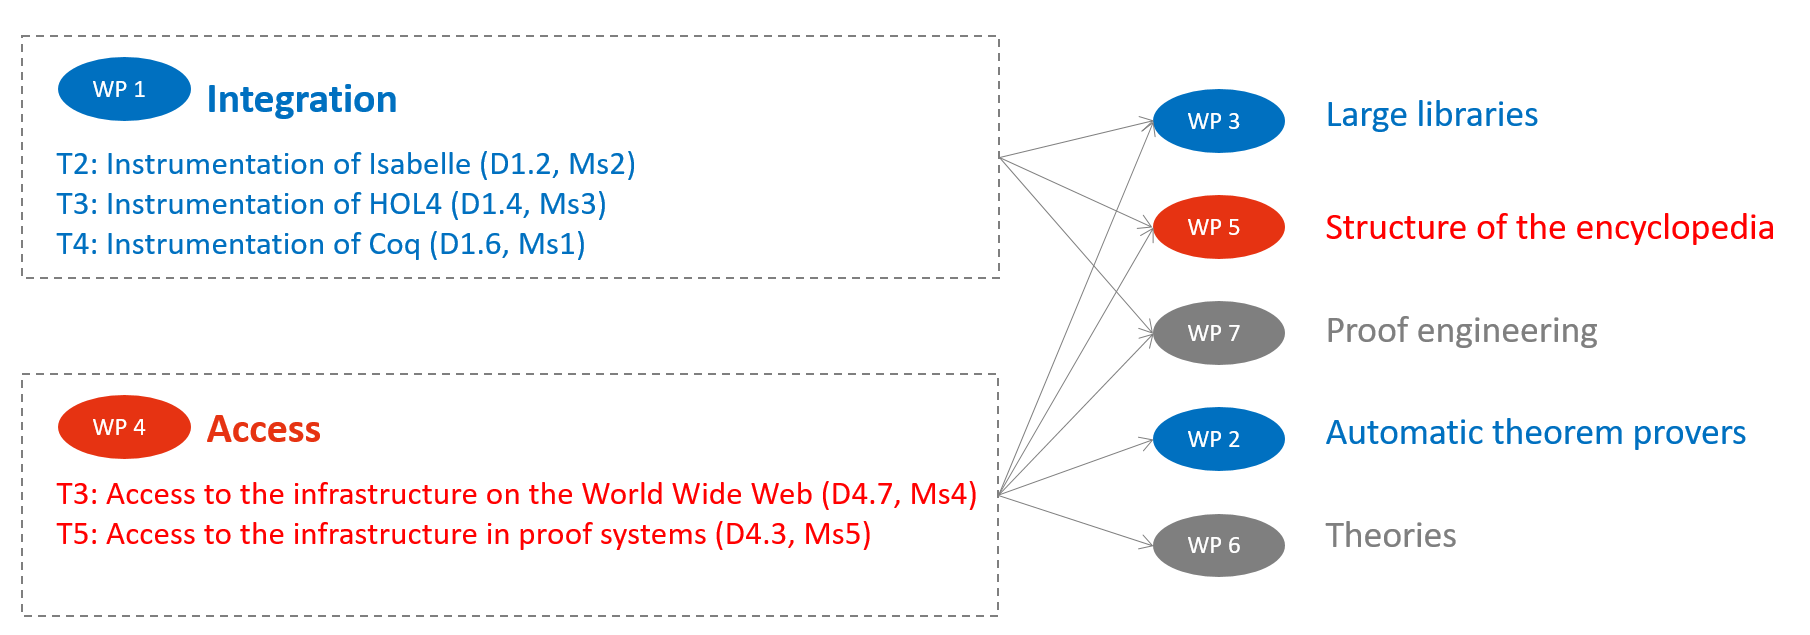
\includegraphics[width=\textwidth]{img/PERT}


%%% Local Variables:
%%%   mode: latex
%%%   mode: flyspell
%%%   ispell-local-dictionary: "english"
%%% End:


\subsection{Work Package List}\label{sec:wplist}

%\makeatletter\wp@total@RM{management}\makeatother
\wpfigstyle{\footnotesize}
\wpfig[pages,type,start,end]

\subsubsection*{List of all deliverables}\label{sec:deliverables}

Here is an overview of the deliverables 
of the work packages. 

%In the table below, \emph{integrating work deliverables} (see top of
%section~\ref{sec:wplist}) are printed in boldface to mark them. They integrate
%contributions from multiple work packages.

{\footnotesize\inputdelivs{8cm}}

%%% Local Variables: 
%%% mode: latex
%%% TeX-master: "propB"
%%% End: 


\subsection{Work Package Descriptions}\label{sec:workpackages}
\begin{workplan}
  \begin{workpackage}[id=instrumentation,wphases=0-48,type=RTD,
  short=Instrument Provers,% for Figure 5.
  title=Instrument proof systems to produce Dedukti proof,
  lead=ISa,
  ISaRM=10]
  
\ednote{MK: We need one coordinating site. original coordinators: Frédéric Blanqui and
  Jesper Cockx}
\ednote{MK: interested parties (add their sites and RM here): David Deharbe,
Tobias Nipkow, Guillaume Genestier, Jesper Cockx, Guillaume Burel, Filip Marić, Makarius
Wenzel, Helmut Schwichtenberg, Nicolas Magaud, Gaspard Férey, Ulf Norell}

\begin{wpobjectives}
  The objective of this work package is to \ldots

This includes notably:
  \begin{compactitem}
  \item \ldots
  \end{compactitem}
  A key aspect will be to foster \ldots
\end{wpobjectives}


\begin{wpdescription}
We know how to express in Dedukti the theories implemented in Matita,
HOL Light, FoCaliZe, Coq, Agda, Lean, Minlog, Isabelle, HOL4,
Atelier B, and Rodin. The systems Matita, HOL Light, FoCaliZe, and
Coq, already have been instrumented to export proofs that can be
checked in Dedukti. Our first work package is to do the same thing for
Coq, Agda, Lean, Minlog, Isabelle, HOL4, Atelier B, and
Rodin. Three methods have to be used here: some of the systems
(Automath style), such as Coq, Agda, Lean, and Minlog already have
proof-terms that can be output, thus the main task is to translate
these proofs into the Dedukti format. Others (LCF style), such as
Isabelle and HOL4, have an inference kernel that can be
instrumented, and often already has, the main task here is to transform
the internal proof-object into an external proof-term. Others, such as
Atelier B and Rodin are slightly more difficult to address. For those,
we need to use the water ford method: extract an incomplete trace (a
sequence of lemmas) and fill the gap using automated theorem proving,
as experimented with Atelier B and Zenon.
\end{wpdescription}

\begin{tasklist}
\begin{task}[id=agda,title=instrument Agda]
[G\"oteborg, Delft]

Agda is a popular dependently typed programming language / proof
assistant based on Martin-L\"of’s intuitionistic type theory. Its theory
is similar to Coq and Lean, but is more focused on interactive
development and direct manipulation of proof terms (in contrast to
using a tactic language to generate the proof terms). Agda has a
sizable standard library (available at
https://github.com/agda/agda-stdlib) that consists of both utilities
for programming and mathematical proofs.


In the summer of 2019, Guillaume Genestier worked together with Jesper
Cockx on the implementation of an experimental translator from Agda to
Dedukti during a research visit at Chalmers University in Sweden. This
translator is still work in progress, but it is already able to
translate 142 modules of the Agda standard library to a form that can
be checked in Dedukti. This exploratory work uncovered several
challenges and opportunities for further work, which are outlined
below.

(1) To support the construction of proof terms, Agda provides powerful
features such as dependent pattern and copattern matching, eta
equality for functions and record types, and definitional proof
irrelevance. The first one – dependent pattern matching – can be
translated directly to rewrite rules in Dedukti. However, the two
latter features – eta equality and irrelevance – rely on Agda’s
type-directed conversion algorithm, while Dedukti’s conversion is
untyped. Hence in order to translate Agda proofs to Dedukti these
features need to be encoded.

One particular concern with the encoding of eta-equality is that in
general it requires storing of additional type information in the
proof terms. It can hence lead to a large blow-up in the size of those
proof terms, and thus greatly increase the cost of typechecking. The
same problem also occurs in other parts of Agda; for example
constructors of parametrized datatypes do not store the values of the
parameters, but they need to be reconstructed in the translation to
Dedukti. We plan to investigate two possible approaches to this
problem: either we can try to find a better encoding which reduces the
size of the type annotation, or alternatively we can extend the
Dedukti language with type-directed conversion rules to render the
type annotations unneccessary.

(2) Another unique feature of Agda is the support for first-class
universe level polymorphism. In particular, Agda has a built-in type
of levels that has complex structure of (in)equality between
levels. Compared to universe polymorphism in Coq, an additional
challenge is that levels in Agda can contain arbitrary terms as
subexpressions. Our plan is to define a sound and complete embedding
of Agda’s level type in Dedukti, based on the existing 1work on
encoding AC (associative-commutative) theories. This would both serve
as a stress test of how well Dedukti can handle complex equational
theories, and improve our understanding of type theories with
first-class universe level polymorphism, which would be useful for the
implementation of Agda.

(3) In contrast to Coq and Lean, Agda does not have a well-defined
core language to which proofs are elaborated. Instead, definitions are
translated to an internal representation that is relatively close to
the user input. This provides a challenge when translating Agda proofs
to Dedukti: each feature in Agda’s internal syntax needs to have its
own translation. As part of this project, we will hence investigate
possible designs for a core language for Agda. Having such a core
language would have several benefits: it would deepen our
understanding of the Agda language, it would increase the
trustworthiness of Agda proofs, and it would make it much easier to
export Agda terms to other languages (such as Dedukti in the context
of this project).

(4) Agda provides an experimental option for extending the language
with user-defined rewrite rules, which are very similar to the rewrite
rules provided by Dedukti. Because of this similarity, we expect it to
be straightforward to translate rewrite rules from Agda to
Dedukti. However, by comparing the two implementations we hope to gain
new insights and find opportunities for improvement on both sides. The
interest of some of these features goes beyond just the Agda
language. In particular, Lean also supports definitional proof
irrelevance, as does Coq with the recent addition of the SProp
universe. Hence we plan to collaborate with the teams working on those
languages to improve the support for these features where there is
overlap.

One research engineer at Chalmers, and one PhD student or postdoc at TU Delft.

Question: does this task belong to WP1 or WP2?


\end{task}

\begin{task}[id=lean,title=Instrument Lean]
[?]
\end{task}

\begin{task}[id=minlog,title=Instrument Minlog]
[LMU München]

The Minlog system <http://minlog-system.de> implements a theory of
computable functionals (TCF, cf. [SchwichtenbergWainer12], Ch.7).).
It is a form of higher order arithmetic where partial functionals are
first-class citizens.

The intended model of TCF is the Scott-Ershov model $C$ of partial
continuous functionals [Ershov77].  Computable functionals are defined
by so-called computation rules, a form of (possibly non-terminating)
defining equations understood as left-to-right conversion rules.  An
important example is the corecursion operator, which is needed to
define functions operating for instance on streams of signed digits (a
convenient format to represent real numbers).  The logical framework
allows to declare a proven equality as a rewrite rule.  Now it is
tempting to identify two terms or formulas when they have the same
normal form w.r.t. rewriting (including of course beta-conversion);
this is often called deduction modulo rewriting.  However, in a setup
like TCF where non-termination is allowed we cannot use normal forms,
but we can consider two terms or formulas as identical when they have
a common reduct.  This drastically simplifies proofs involving real
number arithmetic.

Another central feature of TCF (and hence the Minlog system) is that
it internalizes a proof-theoretic realizability interpretation (in the
form of Kreisel's so-called modified realizability, with realizers of
higher type).  More precisely, for every (co)inductive predicate we
have another one with one argument more, denoting a realizer.  It is
important that this realizers is expressed in the term language of TCF
(an extension of G\"odel's system $T$).  Since a realizer can be seen as
a program representing the computational content of a constructive
existence proof (expressing that a certain specification has a
solution), we now can reason about such programs in a formal way,
inside TCF.  In fact, given a proof M in TCF of a specification all x
ex y A(x,y) we can extract a term (program) t$_M$ and automatically
generate a new proof of all x A(t$_M$(x)).  In other words, for
programs generated in this way from existence proofs, formal
verification is automatic.  Note that for a proof involving
coinduction the extracted term contains the (non terminating)
corecursion operator.  Of course, for efficient evaluation in a second
step we want to translate our extracted term into an efficient
(functional) programming language like Haskell.

Other aspects of Minlog are more common.  It is a proof system in
Gentzen-style natural deduction and therefore based on proof terms
(the so-called Curry-Howard correspondence).  We distinguish between
(co)inductive predicates with and without computational content; in
fact, computational content only arises from (co)inductive predicates
marked as computationally relevant (c.r.).  In particular, both
universal und existential quantifiers do not influence computational
content: one needs to relativize them to c.r. predicates (like
totality) to make them computationally relevant.

A central application area of Minlog is to formalize Bishop-style
[Bishop67] constructive analysis and extract interesting algorithms
from proofs. An example is the Intermediate Value Theorem treated in
[LindstroemPalmgrenSegerbergStoltenberg08].  More recently we have
extracted algorithms operating on (both signed digit and Gray-coded)
stream-represented real numbers from proofs which never mention
streams.  They come in by relativizing real number quantifiers to
appropriate coinductive predicates [Berger09].

The work planned to be done by the Minlog group is to extend this kind
of work further into constructive analysis, e.g. Euler's existence
proof of solutions of ODEs.  We would like to learn from the
experience of other proof assistant developers working on related
matters, both conceptually and by sharing libraries.  It would be very
helpful if this can be done in a unified setting where different
approaches can be compared.

Here we need to go a little futher and propose to express Minlog
proofs in Dedukti.

One Postdoc and one Phd position

\end{task}

\begin{task}[id=isabelle,title=Instrument Isaabelle]
[TU München]

Isabelle as a logical framework \cite{paulson700} is an intermediate
between Type-Theory provers (like Coq or Agda) and classic LCF-style
systems (like HOL Light or HOL4). The inference kernel can already
output proofs as $\lambda$-terms on request, but this has so far been
only used for small examples \cite{Berghofer-Nipkow:2000:TPHOL}. The
challenge is to make Isabelle proof terms work routinely for
reasonably big entries from The Archive of Formal Proofs
\cite{isabelle-afp}. Preliminary work by Wenzel (2019) has
demonstrated the feasibility for relatively small parts of
Isabelle/HOL: some orders of magnitude in scalability are still
missing.

This work package will revisit important aspects of the Isabelle/HOL
logic implementation on top of the Isabelle/Pure framework, such as
normalization of proofs, efficient type-class reasoning, special
representation of derived rules and definition principles (datatypes,
recursion, induction). The volume of proof term output may be reduced
further, by taking more structure of the target language (Dedukti)
into account and omitting certain low-level reasoning of HOL (e.g.\
for inductive types). [Subcontracted to Makarius Wenzel, Augsburg,
Germany.]

The underlying Isabelle/ML implementation platform (on top of Poly/ML)
will be revisited as well, to improve monitoring of memory usage, and
to double the standard heap size from 16\,GB to 32\,GB (without
suffering from the full overhead of the 64\,bit
addressing). [Subcontracted to David Matthews, Edinburgh, UK.]

\end{task}

\begin{task}[id=HOL4,title=Instrument HOL4]
[G\"oteborg]

The HOL4 proof assistant is home to a few medium to large scale
specifications and associated proof developments that have value
outside of HOL4. These specifications include the formal semantics of
the CakeML language (and its verified compiler) and an extensive
specification of the ARM instruction set architecture (ISA) as
formalised by Anthony Fox at the University of Cambridge.

HOL4 has support for exporting proofs to the OpenTheory proof exchange
format, and there has been some work on importing OpenTheory proofs
into Dedukti. However, the current state of these techniques and their
implementations does not scale to real examples such as those
mentioned above.

This part of the project will be about re-thinking and re-designing
the tools HOL4-to-OpenTheory and OpenTheory-to-Dedukti tools such that
they scale to the point where real examples of interest, such as those
mentioned above, can be exported.

2 Person Years at Chalmers


 \end{task}

\begin{task}[id=atelier-b,title=Instrument Atelier-B]
\ednote{Southhampton, Toulouse, Clearsy writes this}
\end{task}
\begin{task}[id=rodin,title=Instrument Rodin]
\ednote{Southhampton, Toulouse, Clearsy}
\end{task}
\begin{task}[id=matita,title=integrate the translator to Matita in Matita itself and export the full Matita library]
\ednote{Bologna}
\end{task}
\end{tasklist}

\begin{wpdelivs}
  \begin{wpdeliv}[due=3,miles=startup,id=requirements,dissem=PU,nature=DEM,lead=ISa]
      {Requirements Analysis and Synchronization}
\end{wpdeliv}
\end{wpdelivs}
\end{workpackage}

%%% Local Variables:
%%% mode: latex
%%% TeX-master: "../propB"
%%% End:

  \begin{workpackage}[id=theories,type=RTD,wphases=1-48,
  short=Theories,% for Figure 5.
  title= Theories,
  activity=jra,
  lead=Inn,
  BiaRM=70,
  BirRM=3,
  IasRM=5,
  InnRM=12,
  InrRM=83,
  LeeRM=3,
  LmuRM=16,
  MedRM=4,
  ProRM=11,
  RunRM=7,
  wphases=1-48,
  ]

\begin{wpobjectives}
  This work package addresses proof systems that are currently at LIL 0, i.e.\
  whose logic and theories have not yet been expressed in Dedukti. Our
  objective is to bring them to LIL 2 or better over the duration of the
  project so that at least elementary proofs can be exported and checked in
  Dedukti.

  Achieving these goals requires (i) expressing the logics
  that underlie these systems in Dedukti and
  (ii) instrumenting the original proof systems so that they can export proofs
  that can be checked in Dedukti. Much of the work required in this work package
  is of foundational nature.
\end{wpobjectives}
\begin{wpdescription}
  The tasks are presented according to the individual systems. Nevertheless,
  the project addresses cross-cutting concerns and foundational aspects such
  as set-theoretic vs.\ type-theoretic foundations, predicate and dependent
  types, (co-)recursive definitions and (co-)inductive proofs and so on. The
  network established in this project will avoid ``reinventing the wheel'', also
  taking advantage of the experiences of the more mature systems considered in
  \WPref{instrumentation} and of the work carried out in \WPref{atpetc}.
\end{wpdescription}

\begin{tasklist}
% \begin{task}[id=abella,title=Express the theory of Abella in Dedukti,shorttitle=Abella]
%   \ednote{K. Chaudhuri, Saclay}
%   \begin{enumerate}
\item Encoding proofs on finite structures: model checking queries supported by
  Abella's Bedwyr prover rely on the exhaustive exploration of finite structures
  and support quantifier alternation. Representing such proofs in Dedukti
  involves alternating phases of deduction and computation. A particular
  challenge is handling backtracking search, which is different from Dedukti's
  notion of computation as confluent rewriting.
\item Encoding cyclic proofs: Abella's implementation of (co-)induction is based
  on cyclic reasoning with size annotated relations. A representation in Dedukti
  requires extracting explicit invariants from cyclic proofs.
\item Equality and unification: Abella's equality proofs examine complete sets
  of unifiers for terms assumed to be equal, based on a trusted unification
  engine. The unification procedure can be recast as a rewrite system in
  Dedukti, but it remains to derive facts from the unifiability of terms.
\item Support $\lambda$-tree syntax: an encoding of Abella in Dedukti requires
  $\lambda$-terms to be considered modulo $\alpha\beta\eta$-equivalence, which
  is not natively supported. Moreover, for reasoning about the inductive
  structure of terms, Abella provides the $\nabla$-quantifier, which provides a
  challenge for representing the full logic in Dedukti.  
\end{enumerate}

%%%%% OLD TEXT %%%%%
% The usual approach to capturing either Peano and Heyting arithmetics
% is to use various axioms (and an axiom scheme for induction) on top of
% classical and intuitionistic first-order logic.  Indeed, this is the
% approach used in the Dedukti proof checker.


% A different approach to encoding arithmetic has been developed over
% the past 20--30 years, starting with papers by Schroeder-Heister and
% Girard in the early 1990s and extended in a series of papers by
% Baelde, Gacek, McDowell, M, Momigliano, Nadathur, and Tiu.  In this
% new setting, first-order logic is extended by considering both
% equality and the least fixed point operator as \emph{logical
%   connectives}: these logical connectives are not available directly
% in Dedukti.

% This new foundations for arithmetic has been implemented in two
% systems: the automated Bedwyr prover and the interactive Abella
% prover.  While neither Bedwyr nor Abella are as popular as many of the
% theorem provers that are covered by this proposal, there are two
% important reasons to consider incorporating them into the Logipedia
% effort.

% First, the Bedwyr prover is capable of constructing proofs for the
% kind of queries that are part of \emph{model checkers}.  This class of
% provers has not yet been incorporated into Dedukti.  The
% proof-theoretic work behind model checking in Bedwyr should provide
% some of the insights needed for allowing Dedukti to proof check the
% results of model checkers.

% Second, Bedwyr and Abella provide for direct and elegant support of
% meta-level reasoning.  Given that the foundations for Bedwyr and
% Abella have been given using Gentzen's sequent calculus, it was
% possible to enrich their foundations to allow for the treatment of
% binding structures within terms.  As a result, it is possible to
% reason directly on terms representing $\lambda$-terms and
% $\pi$-calculus expressions.  In particular, the Abella prover has
% probably the most natural and compact formal treatment of the
% $\pi$-calculus and its meta-theory when compared to all other attempts
% in any other theorem provers.  More generally, the Abella prover
% should be able to treat the meta-theory of programming and
% specification languages as well as various logics and their
% proofs. While these tasks are not the typical tasks considered by the
% majority of theorem provers within the scope of this proposal,
% meta-theory results do play an important role at times: in fact, the
% ultimate questions as to whether or not a proof checkers (such as that
% used by Dedukti) is correct or not will involve meta-theoretic
% questions.

% We propose to work on the general problem of exporting proofs from
% Abella to Dedukti.  (Since all proofs that are constructed
% automatically via Bedwyr can also be constructed manually within
% Abella, we shall limit our discussion below to Abella only.)  The
% proposed work will serve not only to answer the question of how to
% relate these two different foundations for arithmetic but also to
% allow Abella's particular style of proofs to find applications in the
% wider world of formalized proofs.

% The general problem described above has the following constituent parts.

% (1) Proofs involving searching finite structures. Proofs built for
% model checking problems over finite structures have two different
% kinds of phases.  To illustrate, consider trying to find a specific
% node within a binary tree.  If such a node exists, then the proof
% essentially encodes the path to the node in the tree.  If, however, no
% such node exists, then the proof of that negative fact is essentially
% a computation that exhaustively explores the tree.  Using the Dedukti
% terminology: in the first case, the proof involves several deduction
% steps, while in the second case, the proof involves a pure
% computation. When dealing with model checking problems such as
% simulation (in concurrency theory) and winning strategies (in game
% theory), proofs will involve alternating phases involving either
% deduction or computation.  Since the notion of computation in
% Abella-style proofs involves backtracking search, that style
% computation will be quite different from Dedukti's notion of
% computation as confluent rewriting.

% (2) Extending model checking problems to the general case of infinite
% structures and the associated inductive reasoning methods. Although
% the formal basis of Abella uses least and greatest fixed-point
% combinators and explicit (co-)invariants, the Abella implementation of
% (co-)induction is based on cyclic reasoning using size-annotated
% relations. It is known, in principle, how to convert cyclic proofs
% using annotations to proofs with explicit invariants, but an invariant
% extraction procedure that works in all cases is still missing. Once
% such invariants are available, incorporating them into Dedukti should
% be straightforward in association with part (1).

% (3) Binding structures. Abella, as well as several other computational
% logic systems ($\lambda$Prolog, Isabelle/Pure, Twelf, Beluga, etc)
% make use of the so-called \emph{$\lambda$-tree syntax} (a form of
% \emph{higher-order abstract syntax}, HOAS) approach to represent
% bindings. This approach is further enriched in Abella with the
% $\nabla$-quantifier that allows inductive and co-inductive properties
% to be defined based on the \emph{structure} of $\lambda$-terms. We
% propose to examine encodings of $\lambda$-tree syntax in Dedukti. The
% best approach probably involves extending the underlying theory of
% Dedukti with a quantifier similar to Abella's $\nabla$-quantifier.

% (4) Reflective treatment of unification. One of the features of
% Abella's style of proofs is the use of left-introduction rules for
% equality that exhaustively examine complete sets of unifiers for
% $\lambda$-terms. This is implemented in terms of a unification engine
% that is currently a trusted black box, which complicates any proposal
% for exporting proofs to different implementations of unification or
% equality. In Dedukti the unification procedure can be recast as a
% rewrite system, but it is unclear how to derive reflective properties
% based on the unifiability of terms.

% \end{task}

\begin{task}[id=hott,
  title=Express Cubical Type Theory in Dedukti,
  shorttitle=CuTT,
  lead=Inr, % B. Barras
  InrRM=42, % 36 PhD + 6 in kind B. Barras
  BirRM=3,  % 3 in kind B. Ahrens
  LeeRM=3,  % 3 in kind N. Gambino
  wphases=1-48,
  ]
  \vspace{-5mm}
  \begin{compactitem}
  \item Express 2-Level Type Theory (2LTT) as an object theory in Dedukti, as
    a stepping stone towards encoding more expressive variants of homotopy type
    theory.
  \item Express a core Cubical Type Theory (CubTT) in 2LTT: here, the main challenge is
    that equality in cubical type theory is more expressive than what can be
    expressed through rewrite rules in Dedukti.
  \item Define structures such as cartesian cubical type theory on top of the
    core, and compare these structures.
  \item Import the UniMath library into Dedukti and translate it into Cubical
    Type Theory. The UniMath library extends a version of
    Martin-Löf type theory by the univalence axiom. It provides an interesting
    case study for our encoding of CubTT.
  \end{compactitem}
\end{task}

\begin{task}[id=matching,
  title=Express Matching Logic in Dedukti and instrument the K prover,
  shorttitle=K,
  lead=Ias,
  IasRM=5,
  RunRM=7,
  wphases=1-36,
  ]
  \vspace{-5mm}
  \begin{compactitem}
  \item Express Kore in Dedukti: Kore is the specification language used for
    describing Matching Logic theories in K and will serve as the interface
    between the K prover and Logipedia.
  \item Instrument the K prover to produce detailed proof traces expressed in
    Kore.
  \item Integrate an instrumented automated prover (cf.\ tasks
    \taskref{atpetc}{instrumenting} and \taskref{atpetc}{tracetodedukti}) into
    the K prover for obtaining proofs for the queries generated by the K prover.
  \item Combine the translations into Dedukti from Kore and from the automated
    prover into a single Dedukti proof.
  \end{compactitem}
\end{task}

\begin{task}[id=minlog,
  title=Express the theory of Minlog in Dedukti,
  shorttitle=Minlog,
  lead=Lmu,
  LmuRM=16, % 10 post-doc + 6 in kind H. Schwichtenberg + K. Miyamoto
  wphases=1-30,
  ]
  \vspace{-5mm}
  \begin{compactitem}
  \item Further develop and implement extensional realizability in Minlog as
    a necessary first step for bridging Minlog and Dedukti.
  \item Express the core Minlog logic and proofs in Dedukti, benefitting from
    the work on realizability for exporting programme extraction to Dedukti.
  \item Properly encode coinduction and corecursion in Dedukti: these concepts are
    fundamental to Minlog, for example for representing real numbers as streams of
    digits, but they are not native to Dedukti.
  \item Import a subset of Dedukti into Minlog, apply program development by proof
    transformation, and export back. This will make Dedukti a usable tool for the
    development of proofs and programs in constructive analysis and allow Minlog
    users to benefit from theories formalized using other proof assistants.
  \end{compactitem}
\end{task}

\begin{task}[id=mizar,
  title=Express the theory of Mizar in Dedukti,
  shorttitle=Mizar,
  lead=Bia,   % Artur Korni{\l}owicz
  BiaRM=70, % 48 post-doc + 22 in kind
  InnRM=12,   % 9 post-doc + 3 C. Kaliszyk
  wphases=1-48,
  ]
  \vspace{-5mm}
  \begin{compactitem}
  \item Express the foundations of Mizar (first-order Tarski-Grothendieck set
    theory) in Dedukti, together with Mizar's soft
    type system. Take advantage of Dedukti's rewriting capabilities to automate
    parts of type inference.
  \item Instrument Mizar to export type disambiguation data. Exporting the
    information present in the Mizar types will enable us to optimize the
    representation of Mizar statements in Dedukti.
  \item Express Mizar's equality checking and unification steps as a mix of
    small proof steps and rewrite rules so that Dedukti's proof kernel can
    verify them. Export necessary semantic information that is not currently
    available outside of the Mizar checker in order to check the basis of the
    Mizar library and make it available in Logipedia.
  \end{compactitem}
\end{task}

\begin{task}[id=pvs,
  title=Express the theory of PVS in Dedukti,
  shorttitle=PVS,
  lead=Inr,   % Gabriel Hondet
  InrRM=20,  % 20 in kind G. Hondet
  wphases=1-48,
  ]
  \vspace{-5mm}
  \begin{compactitem}
  \item Extend the existing encoding in Dedukti,
    restricted to a fragment of PVS with decidable type checking, and represent
    proofs of type checking conditions for predicate subtypes.
  \item Instrument PVS to export proof traces to Dedukti given that PVS proof
    tactics do not produce proof terms.
  \item Design and implement a PVS proof checker in Dedukti based on the
    reconstruction of proof traces exported from PVS.
  \end{compactitem}
\end{task}

\begin{task}[id=smart,
  title=Express Smart models and proofs in Dedukti,
  shorttitle=Smart,
  lead=Pro,   % Stephane Lescuyer
  ProRM=11,
  wphases=1-48,
  ]
  \vspace{-5mm}
  \begin{compactitem}
  \item Choose a viable translation strategy from Smil programs (the
    intermediate form of Smart models used by ProvenTools) into Dedukti
    by experimenting with direct translations or translations through a
    different tool such as Coq or Why3.
  \item Develop a prototype capable of translating the definitions and proof
    obligations corresponding to relevant examples from the Smart
    standard library.
  \item Integrate the prototype into ProvenTools: integrate proof rules internal
    to the prover and evaluate the scalability to cross-verifying real-world use
    cases.
  \end{compactitem}
\end{task}

\begin{task}[id=tla,
  title=Express the theory of \tlaplus in Dedukti,
  shorttitle=\tlaplus,
  lead=Inr,   % Stephan Merz
  InrRM=21,   % 18 post-doc + 3 in-kind S. Merz
  MedRM=4,
  wphases=1-48,
  ]
  \vspace{-5mm}
  \begin{compactitem}
  \item Express the untyped \tlaplus set theory with choice in
    Dedukti.
  \item Instrument backends of the \tlaplus Proof System to export proofs,
    taking advantage of Dedukti's rewriting capabilities in order to compress
    the size of proofs.
  \item Formalize a distributed assignment of rehabilitation programs to
    patients and updates of the process in MED-EL's software.
  \end{compactitem}
\end{task}

\end{tasklist}

\begin{wpdelivs}
  \begin{wpdeliv}[due=18,id=wp2midterm,dissem=PU,nature=R,lead=Inn]{Report on defining theories in Dedukti}\end{wpdeliv}

  \begin{wpdeliv}[due=48,id=wp2cubical,dissem=PU,nature=R,lead=Inr,task=hott]{Report on the integration of Cubical Type Theory in Dedukti}\end{wpdeliv}

  \begin{wpdeliv}[due=36,id=wp2matching,dissem=PU,nature=R,lead=Ias,task=matching]{\hspace{-2mm}Report on the integration of Matching Logic}\end{wpdeliv}

  \begin{wpdeliv}[due=48,id=wp2minlog,dissem=PU,nature=R,lead=Lmu,task=minlog]{Report on the integration of Minlog}\end{wpdeliv}

  \begin{wpdeliv}[due=48,id=wp2mizar,dissem=PU,nature=R,lead=Bia,task=mizar]{Report on the integration of Mizar}\end{wpdeliv}

  \begin{wpdeliv}[due=48,id=wp2pvs,dissem=PU,nature=R,lead=Inr,task=pvs]{Report on the integration of PVS}\end{wpdeliv}
  
  \begin{wpdeliv}[due=48,id=wp2smart,dissem=PU,nature=R,lead=Pro,task=smart]{Report on the integration of Smart}\end{wpdeliv}
  
  \begin{wpdeliv}[due=48,id=wp2tlaplus,dissem=PU,nature=R,lead=Inr,task=tla]{Report on the integration of \tlaplus}\end{wpdeliv}
\end{wpdelivs}
\end{workpackage}


%%% Local Variables:
%%% mode: latex
%%% TeX-master: "../propB"
%%% End:

  \begin{workpackage}[id=libraries,wphases=0-48,type=RTD,
  short=Libraries,% for Figure 5.
  title=Libraries,
  lead=Inr,
  InrRM=10,
  TumRM=39]
%TUM: 24 for Analysis library, 12 for CakeML,
%TUM: 3 for AFP/Makarius (25k EUR) - the latter do not generate overheads!


\ednote{MK: We need one coordinating site. original coordinators: Georges Gonthier and
Tobias Nipkow} \ednote{MK: interested parties (add their sites and RM here): David
Deharbe, Nicola Gambino, Tobias Nipkow, Makarius Wenzel, Julien Narboux, Gaspard Férey,
François Thiré, Magnus Myreen}

\begin{wpobjectives}
The objective of this WP is to export large dedicated libraries in curated form to Dedukti
for access to end-users. The focus is \emph{Access} and \emph{Scalability}.
\begin{compactitem}
\item This WP is responsible for supplying the lion's share of proofs for
the Dedukti data base.  As a result it will be a stress test for the
results of \WPref{instrumentation}: is the proof infrastructure
capable of processing truly large amounts of material/proofs?

\item The target libraries are dedicated to particular application
areas. They provide a substantial coverage of that application area
and do so in a structured manner. This may require reworking the
libraries for better access.

\item The libraries are curated for end-user application. That is, they
are structured according to application specific ontologies that
support browsing and search. The structuring leverages the
infrastructures of \WPref{structuring} and will be a
stress test for the results of \WPref{structuring}: is the metadata
infrastructure capable of representing the structure of large
libraries?
\end{compactitem}
\end{wpobjectives}


\begin{wpdescription}
Translating the standard libraries of the systems is part of the \WPref{instrumentation}.
This WP focusses on advanced libraries selected according to the following criteria:
\begin{compactitem}
\item Relevance: the libraries should support core areas of matematics and computer science.
\item Coverage: the libraries should have a wide coverage of an application area.
\item Maturity: the libraries should have been used in a significant application already.
\end{compactitem}
As a result we selected the following libraries: MathComp, Coq's revised
Analysis library, the Archive of Formal Proofs, Isabelle's revised Analysis and Probability library,
GeoCoq, Flyspeck and CakeML. In the future we plan to incorporate
CompCert, seL4, and selected Mizar and PVS libraries (once Mizar and
PVS have reached LIL 2).
\end{wpdescription}


\begin{tasklist}
\begin{task}[id=mathcomp,title=MathComp]
\ednote{Sophia, Saclay (Gonthier), Paris}
\end{task}

\begin{task}[id=milc,title=Revised Coq Analysis Library]
\ednote{Saclay (Boldo), Paris, Sophia}
\end{task}

%\begin{task}[id=mizar,title=The Mizar library]
%\ednote{Innsbruck, Bialystok}
%\end{task}

\begin{task}[id=afp,title=Isabelle's Archive of Formal Proofs]
\ednote{TU München (Wenzel)}

Isabelle's Archive of Formal Proofs (AFP) \cite{isabelle-afp} is a
growing user-contributed online library for Isabelle. In Feb-2020, the
AFP consisted of more than 500 entries (articles of formalized
mathematics) by 340 authors, and required approx. 60h CPU time for
checking (using many gigabytes of memory).  The purpose of this task
is to scale up the Isabelle instrumentation for Dedukti further, to
cover major parts of this library. We do not intend to restructure or
document the library further beyond what is provided by the authors of
each article and by the hierarchical dependencies among the articles.

The key challenge is scaling. The ultimate aim is to export the main
substance of the AFP without promising full coverage: some entries
with prohibitive resource requirements will be omitted. Also note that
the AFP is continuously growing at a high rate and thus a moving
target.
\end{task}

\begin{task}[id=isaAnalysisProb,title=The Isabelle Analysis \& Probability library]
\ednote{TU München (Nipkow)}

The Isabelle Analysis and Probability Theory library consists of more than
200.000 lines of definitions and proofs, corresponding to almost 4000 printed
pages. It covers topology, homology, multivariate, functional and complex
analysis, measure and probability theory, and a dedicated library for
ordinary differential equations. It is fair to say that it is the most
advanced machine-checked library in the area of analysis and probability
theory.\footnote{The Isabelle analysis and probability theory library is
in part based on the extensive library of the HOL Light system but has
generalized it from real numbers to appropriate algebraic structures and
includes areas absent from the HOL Light library (in particular measure
theory and ordinary differential equations).} It is currently used by 60 out
of 500 articles in the Archive of Formal Proofs, a user-contributed library
of Isabelle/HOL proofs from all areas of computer science and
mathematics. Moreover, it is the only existing library in this area where
proofs are structured and readable. Due to its size and generality and
because analysis and probability theory are pervasive in any application in
the engineering and natural sciences and economics, this library will be a
KER of the project: it is a fundamental enabling resource for almost any
formal verification activity in these areas, for example autonomous driving
and mathematical finance. The purpose of this task is to structure, document
and develop this library for optimal accessibility, ease of use and
comprehensiveness. The aim is a curated library for applications.

Any library is only as useful as its structure and documentation, no matter
how sophisticated the search facilities are. Therefore the primary aim of
this task is to make this library easily accessible. At the same time the
library needs to be developed further: some material needs revising for ease
of use and some essential material needs to be added.

\textbf{Accessibility}\quad
The library is a large collection of theories with a hierarchical dependency
relation. However, this structure has grown over time and does not always
reflect the abstract mathematical dependencies. In short, the structure needs
to be modularized. This requires a significant refactoring effort.
%
At the same time we need to add metadata to the source material to turn this
structured collection of theorems and proofs into a curated library at the
Dedukti level.  This is where we need to interface with \WPref{structuring}. We
will be test drivers of the metadata infrastructure provided by that WP, in
particular the ability to describe ontologies for structuring in the large.
This will also entail annotating those statements in the library that
correspond to proper mathematical theorems as opposed to auxiliary lemmas
required only for the benefit of the theorem prover.
To increase accessibility we will also include links from the library into
Wikipedia and in particular in the other direction to raise the awareness
of Dedukti.

\textbf{Development}\quad
Although the library support for integrals is extensive, it suffers
from the (necessary) coexistence of different kinds of
integrals. This complicates proofs about integrals in applications and needs
to be unified, which entails further refactoring. The rest of the
development adds further essential material:
1. Fourier analysis because of its extreme important both for pure mathematics and for
engineering and physics (especially the Fourier
transform). A formalization of basic properties of the Laplace transform is already available in the AFP. 2. Stability theory for differential equations and
dynamical systems, in particular Lyapunov functions, because of their
relevance for the verification of cyber-physical systems.
3. Stochastic differential equations to model a large range of
dynamical systems with stochastic components, from physics to financial markets.
\end{task}

\begin{task}[id=geocoq,title=The GeoCoq library]
\ednote{Sophia (Boutry), Strasbourg, Belgrade}
\end{task}

\begin{task}[id=flyspeck,title=The Flyspeck library]
\ednote{Saclay (Grienenberger)}
The
\textsc{HOL Light} library is especially large and varied.
    
First, its standard library contains definitions of the logical connectives,
pairs, natural and real numbers, well-founded relations, lists, sets, and usual
results concerning these objects. The standard library also contains tools to
define inductive types, iterate operations, execute calculations over natural
and real numbers, integers, and rationals. Many more libraries are added to
this basis, formalizing many mathematical fields, objects, and results, for
example arithmetics, complex numbers, group and ring theory, orderings, first
order logic, Hilbert axiomatic geometry, complex function vector spaces,
geometric algebra, quaternions, IEEE floating-point numbers, Jordan curves.

One of those libraries, particularly large and unique, is the multivariate
analysis library
\footnote{\url{https://github.com/jrh13/hol-light/tree/master/Multivariate}},
which spans the fields of metric spaces, topology, homology, linear algebra,
convexity, real and complex analysis and transcendentals, derivatives, and
integration. This profusion of multivariate analysis theorems was partly
motivated by the \textsc{Flyspeck} project.

The \textsc{Flyspeck} project gives a formal proof of the \textsc{Kepler}
conjecture. The statement and proof is based on an original proof of Thomas
\textsc{Hales} \cite{DBLP:journals/corr/HalesABDHHKMMNNNOPRSTTTUVZ15},
and entirely formalized and proved in \textsc{HOL Light}
\footnote{\url{https://github.com/flyspeck/flyspeck}}.
    
This variety and multitude of formalized mathematical results, sometimes unique
to this system, motivates the project of importing the \textsc{HOL Light}
library and \textsc{Flyspeck} project in the \textsc{Dedukti} system, in view
of its integration into \textsc{Logipedia}.
 
Proofs coming from the HOL systems, including \textsc{HOL Light}, are known to
be very large, adding to the already existing issue of the scalability of
exporting software for large libraries
\cite{DBLP:conf/tphol/Wong95,DBLP:conf/cade/ObuaS06,DBLP:conf/itp/KellerW10,
DBLP:conf/cade/Kumar13}. As an example, the size of the standard library is
1.5M in \textsc{HOL Light} files (i.e. .ml files), while the same files once
exported as \textsc{Dedukti} files scale to 2G, and the whole
\textsc{HOL Light} library and the \textsc{Flyspeck} project are each as
large as 30M. The multitude of automatic tactics and their increasing
complexity and number of dependencies suggests that the generation time, size,
and rechecking time of exported proofs will not increase linearly. Scalable
export techniques \textsc{HOL Light} proofs have been investigated
\cite{DBLP:conf/itp/KaliszykK13} and can provide a solid base to
this project; for want of significantly reducing the size of generated
\textsc{Dedukti} files, the time of export could at least be reduced.

The main milestones of this task are the further automation of the translation
from \textsc{HOL Light} to \textsc{Dedukti}, the import of the multivariate
analysis library, the import of the whole \textsc{HOL Light} library, and the
import of the \textsc{Flyspeck} in \textsc{Dedukti}.
\end{task}

\begin{task}[id=cakeml,title=The CakeML compiler library]
\ednote{Chalmers (Myreen), Strasbourg, TU München}
The CakeML compiler library consists of the CakeML programming language
definition, its compiler and the correctness proofs about the
compiler. This is a cutting edge compiler library and one of only two
verified compilers for real languages, the other being CompCert. Its
export to Dedukti is one of the KERs of this project. Because of the
size and importance of this library, we will approach the export from
two angles.

The first approach utilizes OpenTheory-based technology. The CakeML
compiler development lives within the HOL4 prover. HOL4 can export
definitions and proofs in the OpenTheory format, which can in turn be
translated into Dedukti. This link from HOL4 via OpenTheory to Dedukti
exists but, in its current state, fails to scale to the task of
transporting something as sizeable as the CakeML compiler
development. This part of this task will rework the route via
OpenTheory to scale better, possibly taking inspiration from an
OpenTheory-like approach that scaled well for the HOL light
prover~\cite{KaliszykK13}.

The second approach establishes a connection from HOL4 via Isabelle to
Dedukti. The basis is a promising new approach of virtualizing HOL4
inside Isabelle \cite{ImmlerRW19}. That is, the inference
kernel of HOL4 is replaced by that of Isabelle and the resulting
system produces Isabelle theorems instead of HOL4 theorems. This has
the invaluable additional benefit that tools, not just theorems, can
be shared. As a benchmark of the viability of this approach we plan to
export CakeML via Isabelle to Dedukti.
\end{task}

By Arthur Chargueraud
{\bf Trusted chain}

A grant challenge in program verification is that of running trusworthy
software on trustworthy hardware. This challenge can be decomposed in
four steps: (1) formally verify the source code of the program,
(2) compile this code using a formally-verified compiler,
(3) launch the program on a formally-verified operating system,
(4) running the whole thing on hardware with formally-verified circuits.

Developing a program verification framework, a verified compiler, a
verified operating system, and a verified hardware, corresponds to 4
daunting tasks. Just setting up a reasonable proof-of-concept takes of
the order of 10 man-year of work. Raising the bar to a production-ready
tool takes at least Can additional order of magnitude in terms of efforts.

Considerable progress has been made on these three aspects
over the past decade, and every year the technology becomes more mature.
Yet, there is a pitfall. The tools are not all developed using the same
theorem prover, not just for historical reasons but also because different
proof assistants have appeared better-suited at different tasks.

In that setting, how one could possibly complete a trustworthy chain if
the four main pieces of the chain are not properly hooked to one another?
As a concrete example, CFML is a program verification for verifying ML code,
developed in Coq; and CakeML is a verified compiler for ML code,
developed in HOL4. How can we combine the two tools to produce verified
machine code from verified ML code?

There are two main ways to address the issue. One way is to port the
proofs of all the formalized tools into a same proof assistant.
Doing so might be possible in a far future, however given the scale and
the complexity of the tools, this approach does not provide a short-term
solution. Another, more accessible approach consists of translating
between proof assistants only the formal statements associated with the
interfaces between the 4 pieces of the verified chain.

Concretely, the interfaces involve: (1-to-2) a formal semantics for
a programming language, (2-to-3) a formal semantics for a set of
system calls (the OS API and isolation model), (2-and-3-to-4) a formal
semantics for machine code (instruction set and memory model).
Translating such formal interfaces, which consists solely of statements,
is considerably easier than translating all the verification proofs
associated with the tools.

A proposal for translating such interfaces should satisfy the following
requirements. First, the translations must to be trusworthy. In particular,
translation by hand is not an option, and developing translation tools
between every pair of provers might make the trusted code base prohibitively
large. Second, the translations should be maintainable. Indeed,
formal specifications of the aforementioned interfaces do evolve, slowly but
surely, through time, in particular for incorporating new features.
Third, the translations should produce formal definitions that are written
in a style sufficiently idiomatic with respect to the target proof assistant.
Indeed, carrying out proofs with respect to definitions in non-idiomatic
style induce prohibitive overheads.

We propose to tackle the problem by leveraging the unifying language
Dedukti in the following way. Assume that we have, for formal statements,
a bi-directional translations between each prover and Deduki. Then,
we could translate a formal interface from one system to another.
The user may then provide alternative, more idiomatic statements for
specific definitions, and prove (by hand) that the alternative definitions
are equivalent to the automatically-generated ones. If the original
interface is modified, then the automatic translations can be updated,
and the proof system would notify the user of which alternative definitions
need to be updated accordingly.

For example, we could take CakeML's semantics of its input ML language,
translate it automatically into Dedukti, then translate Dedukti's
definition into Coq, refine by hand a few definitions to make them more
idiomatic, and obtain a usable Coq semantics, with respect to which
the correctness of the CFML verification tool can be established in Coq.
Completing this case study is motivating not only because it delivers
an immediate result of relating two existing tools, but also because it
would validate the general approach of translating semantics via Dedukti
in a realistic manner.

Beyond this one example, other motivating case studies will be considered,
such as translating the formal semantics of ComCert-C into other proof
assistants, or translating the formal semantics of ARM instruction set.

%\begin{task}[id=unimath,title=The UniMath library]
%\ednote{Birmingham (Ahrens)}
%\end{task}

%\begin{task}[id=pvs,title=The NASA PVS library]
%\end{task}
%\begin{task}[id=sel4,title=The seL4 library]
%\end{task}

%\begin{task}[id=compcert,title=The CompCert library]
%\end{task}
\end{tasklist}

\begin{wpdelivs}
  \begin{wpdeliv}[due=3,miles=startup,id=requirements,dissem=PU,nature=DEM,lead=Inr]
      {Requirements Analysis and Synchronization}
\end{wpdeliv}
  \begin{wpdeliv}[due=36,miles=isabelle-stdlib,id=requirements,dissem=PU,nature=DEM,lead=Tum]
      {Scalable export of proof terms for major parts of Isabelle/AFP}
  \end{wpdeliv}
\end{wpdelivs}
\end{workpackage}

%%% Local Variables:
%%% mode: latex
%%% TeX-master: "../propB"
%%% End:

  \begin{workpackage}[id=atpetc,wphases=0-48,type=RTD,
  short=ATPs etc.,% for Figure 5.
  title={ATP, SAT, SMT, Model checkers},
  lead=Lie,
  LieRM=10]

\ednote{MK: interested parties (add their sites and RM here): Guillaume Burel, Raphaël Cauderlier, David Deharbe, Pascal Fontaine, Emilio J. Gallego Arias, Olivier Hermant, Cezary Kaliszyk, Chantal Keller, Filip Marić, Stephan Merz, Dale Miller, Julien Narboux, Martin Suda, Josef Urban}

\begin{wpobjectives}
  The objective of this work package is to \ldots

This includes notably:
  \begin{compactitem}
  \item \ldots
  \end{compactitem}
  A key aspect will be to foster \ldots
\end{wpobjectives}


\begin{wpdescription}

  The aim of this work package is to connect automated tools to the Logipedia
  infrastructure.

% https://annuel2.framapad.org/p/9ef1-logipedia?lang=fr
% https://lite.framacalc.org/9f0a-logipediawp4

The importance of proofs in automated theorem provers, satisfiability
modulo theories solvers, propositional satisfiability solvers and
model checkers is increasingly recognized.  While for the
propositional case, the community agrees on a well defined proof
format, the situation is not clear for the other kinds of automated
reasoners.  There is no clear format for SMT, and the TSTP format for
automated theorem provers fixes a syntactic template for proofs rather
than providing an unambiguous framework to express proofs
semantically.

Some preliminary works predating this proposal clearly establish that
Dedukti can accommodate proofs in Satisfiability Modulo Theories,
automated theorem provers, and SMT.  In this work package, we will
build on those preliminary work and provide a set of conduits from the
established formats used in automated tools. For the tools that do not
have yet an established format, we will make a selection of tools
(Zipperposition and E for automated theorem provers, CVC4 and veriT
for SMT, ??? for model checking) and provide a conduits for those
tools.  These conduits and the techniques used in the embedded
translation will be properly documented, to ease integration of
further tools of the kind.  If a standardized proof format appears for
some kind of tools, the conduits will be updated to adopt the new
standard.

In this work package, we also plan to integrate in Logipedia some
well-chosen proofs coming from automated tools.  Well-chosen proofs
will have to be representative of typical applications of the tools,
and be of reasonable size.  They will serve as examples to the
community, to illustrate the potentials of Dedukti and Logipedia.


Create the infrastructure to enable the long term goal: be able to split a large proof
obligation into smaller parts and distribute to the appropriate automatic engines, that
would all produce proofs, glued together in a single large proof for the original proof
obligation.
\ednote{Nancy, Liège}
\end{wpdescription}


\begin{tasklist}
\begin{task}[id=instrumenting, title=Instrumenting ATPs to produce
  traces]
  Task leader: Pascal Fontaine
  % WP Leader supervision: Pascal
  % Participants
  % Stephan Schulz
  % Martin Suda
  % Guillaume Bury (OCamlPro)
  % Guillaume Burel
  % Julien Narboux
  % Pedro Quaresma
  % Predrag Janicic
  % Resources: One PhD student shared bw Schulz and Fontaine
  % Albin Coquereau (OCamlPro)
  % Sylvain Conchon (OCamlPro)
  % François Bobot (Why3)
  
Considered provers:
\begin{itemize}
\item Cubicle (OcamlPro, Guillaume Bury, Sylvain Conchon)
\item provers for geometry (Julien Narboux and Pedro Quaresma)
\item coherent logic theorem prover (Predrag Janicic)
\item SMT (alt-ergo, veriT: Pascal Fontaine)
\item FOL ATPs (Pascal Fontaine, Stephan Schulz)
\item \dots
\end{itemize}

traces from SAT: understood

traces from SMT: still some gaps, about arithmetic, preprocessing.  Engineering issue too because of the amount of code that is involved

traces from geometry solvers: seems to be a good candidate, because the proof process is suitable to produce traces

traces from FOL: there is a format, and mainstream solvers do follow the standard format, but proofs are coarse grained

traces from HOL provers: strongly relates to FOL

\end{task}


\begin{task}[id=tracetodedukti, title=Translate ATP traces into Dedukti]
  Task leader: Guillaume Burel
  % Pascal Fontaine
  % Chantal Keller
  % Martin Suda
  % Guillaume Bury (OCamlPro)
  % Guillaume Burel
  % Julien Narboux
  % Pedro Quaresma
  % Predrag Janicic
  % Resources: One PhD student shared bw Schulz and Fontaine
  % Albin Coquereau (OCamlPro)
  % Sylvain Conchon (OCamlPro)
  % François Bobot (Why3)

As pointed out in Task~\localtaskref{instrumenting}, it is easier to
instrument provers to make them output traces instead of directly
provide Dedukti proofs. The goal of this task is to reconstruct the
proof traces in order to build Dedukti proofs from them. The proposed
process is the following: each step of the trace is transformed into
an independent subproblem; each of these subproblems is given to a
prover that can output Dedukti proofs; proofs of the subproblems are
then combined to produce a global proof of the original problem. Since
subproblems correspond to atomic steps of the proof trace, they are
relatively simple, so that we can hope that the prover producing
Dedukti proofs will not struggle to find a proof. This process is
quite similar to what is done by the hammer tools of interactive
theorem provers (Sledgehammer in Isabelle/HOL, HOLyHammer for HOL4, etc.)
which reconstruct proofs from traces produced by automated theorem
provers.

This scheme has already been prototyped in a tool called
\href{https://github.com/Deducteam/ekstrakto}{Ekstrakto}. Ekstrakto takes a TSTP
file, as can be produced by e.g.\ the provers E and Zipperposition, and it uses
Zenon Modulo and ArchSAT to prove the subproblems. Ekstrakto was designed to be
agnostic w.r.t.\ the prover producing the trace; in particular it does not
depend on the specific set of inference rules of the prover. It was also
designed to be agnostic w.r.t.\ the prover used to prove the subproblems; it is
only required that the prover can output a Dedukti proof in the correct encoding
of first-order logic.

Although Ekstrakto has already shown that it is a
valuable approach, it is work in progress. In particular, the
following issues still need to be addressed:

\begin{compactenum}
  % extension to other proof trace formats
\item Up to now, Ekstrakto can only take traces in TSTP format as input. We plan
  to make it understand traces in other formats, notably traces from SMT
  solvers, as well as all formats developed in
  Task~\localtaskref{instrumenting}.

  Deliverables :
  \begin{itemize}
  \item T+6 a version of Ekstrakto that input traces from SMT solvers
  \end{itemize}

  % unprovable steps

\item  Some steps in the proof traces are not provable: their conclusion is
  not a logical consequence of their premises. However, they preserve
  provability: the original problem has a proof if and only if the
  problem with the conclusion of the step also has a proof. This is the
  case for instance of the Skolemization step in first-order automated
  theorem provers, of the introduction of new definitions, as well as
  the RAT property in traces produced by SAT solvers. The approach of
  Ekstrakto cannot be used here, because the subproblem corresponding to
  the step cannot be proved. However, since provability is preserved, it
  should be possible to transform a
  proof using the conclusion of the step into a proof using its
  premises. Such a transformation depends on the nature of the step that
  has been used. We plan to include in Ekstrakto a way to handle
  Skolemization and definition introduction, which are the two step
  families that are missing to be able to manage all traces from the
  major first-order theorem provers.

  Deliverables :
  \begin{itemize}
  \item T+12 a version of Ekstrakto that handles definition-introduction steps
  \item T+24 a version of Ekstrakto that handles Skolemization steps
  \end{itemize}


  % specialization for theories

\item  Dedukti-producing provers used by Ekstrakto, namely Zenon Modulo and
  ArchSAT, are meant for pure first-order logic. However, we would like
  to deal with proof traces that use some specialized theory,
  e.g.\ arithmetic or bit-vectors, as could be output by SMT
  solvers. Although such theories could be presented as a set of axioms
  in first-order logic, it is almost certain that neither Zenon Modulo
  nor ArchSAT could be able to find non-trivial proofs using these
  axioms. Here, the idea would be to develop small provers dedicated to
  a particular theory, and outputting Dedukti proofs. Such provers would
  be called when a step in the trace relies on said theory. These
  provers need not be very optimized, since trace steps are relatively
  small; this should help producing Dedukti traces. A way to achieve
  this could be to extend Zenon Modulo: indeed, Zenon modulo can find
  proofs modulo arithmetic, but it is not able to produce a Dedukti
  proof yet.

  Deliverables :
  \begin{itemize}
  \item T+36 a prover modulo arithmetic outputting Dedukti proofs
  \item T+48 a prover modulo another theory outputting Dedukti proofs
  \end{itemize}

\end{compactenum}
  Depends on T1.

  One PhD student
  
\end{task}


\begin{task}[id=deduktitoatp, title=Translate Dedukti statements into ATPs inputs]
  Task leader: Guillaume Bury (WP leader contact: Chantal Keller)
  % Guillaume Bury
  % Chantal Keller
  % Pascal Fontaine (SMT-LIB)
  % Josef Urban + Martin Suda (TPTP)
  % François Bobot (Why3)
  
\begin{itemize}
\item encodings into FOL
\item links to WP6: reverse mathematics
\item benchmarks
\end{itemize}

\end{task}


\begin{task}[id=library, title=Logipedia as a source of knowledge for ATP]
  Task leader: Martin Suda (WP leader contact: Pascal Fontaine)

  % Josef Urban
  % Pascal Fontaine
  % Stephan Schulz
  
Depends on T3.

\begin{itemize}
\item A library of known facts for ATPs
\item Lemma selection is crucial
\end{itemize}

Proposition: Add in ACSL (C specification language) an "import from
Logipedia, ..." which allows a user to get the ressources to model the
behavior of its code. The modelisation is at the end used by ATP through
Frama-C-WP.

\end{task}


\begin{task}[id=reconstruction, title=ATPs for Logipedia]
  Task leader: Cezary Kaliszyk (WP leader contact: Chantal Keller)

  % Chantal Keller
  % Josef Urban
  % Martin Suda

  Six month PhD student

\begin{itemize}
\item native provers for Logipedia
\item proof reconstruction
\end{itemize}

\end{task}


\begin{task}[id=readiness, title=Using ATPs to increase Logipedia readiness]
  Task leader: Chantal Keller

  % Guillaume Burel
  % People from other packages?  

\begin{itemize}
\item ATPs can be used to fill the holes in proofs (e.g. PVS)
\item ATPs can be used to fill the gaps between systems and alignments
\end{itemize}

\end{task}


\begin{task}[id=cooperation, title=Make ATPs cooperate]
  Task leader: François Bobot (Contact: Chantal Keller)

  30 h.m

  % François Bobot (Why3)
  % Chantal Keller

\begin{itemize}
\item Why3: gather the proof from the called provers, add traces for the
  Why3 transformations and send all this information to Ekstrakto
\item External preprocessing, add traces to the rewrite engine of
  Frama-C-WP, which is used before sending goals to solvers, and give
  them to Ekstrakto
\item Add in ACSL (C specification language) an "import from Logipedia,
  ..." which allows a user to get the ressources to model the behavior
  of its code. The modelisation is at the end used by ATP through
  Frama-C-WP. (Move to T4?)
\end{itemize}

\end{task}
\end{tasklist}


% \begin{tasklist}
%   \begin{task}[id=tools,title=Automatic Tools Exporting Proofs]
%     %% Guillaume Burel: expertise
%     %% Raphael Cauderlier: SAT/FOL proof checking in Dedukti
%     %% David Deharbe: pr in Atelier B
%     %% Pascal Fontaine: SMT
%     %% Emilio J. Gallego Arias
%     %% Thibault Gauthier
%     %% Olivier Hermant
%     %% Cezary Kaliszyk
%     %% Chantal Keller: expertise in translating proofs from SAT/SMT into other formalisms
%     %% Filip Marić
%     %% Stephan Merz
%     %% Dale Miller
%     %% Julien Narboux
%     %% Martin Suda: FOL ATP
%     %% Josef Urban: FOL ATP
%   \end{task}

%   \begin{task}[id=challenges,title=Logipedia as a Source of Challenges for Automatic Reasoners]
%     %% --> Translation to TPTP, SMT-LIB, DIMACS
%     %% Guillaume Burel: expertise / SAT
%     %% Pascal Fontaine: SMT-LIB
%     %% Cezary Kaliszyk: TPTP
%     %% Julien Narboux: Geometric benchs
%     %% Josef Urban: TPTP
%   \end{task}
%   \begin{task}[id=commang,title=Cooperation of Reasoners via Dedukti/Logipedia]

%     %% Once ITP understand Dedukti and ATP output Dedukti, then the first step of this is trivial
%     %% But many other things can be done within this task: choosing which solver to use, cutting proof obligations into pieces, etc...

%     %% Guillaume Burel: expertise
%     %% David Deharbe: Atelier B
%     %% Pascal Fontaine: SMT ++ ???
%     %% Chantal Keller: Knowledge in combining various ATPs
%     %% Martin Suda: cooperation between FOL ?
%     %% Josef Urban: cooperation between FOL ?
%   \end{task}
%   \begin{task}[id=database,title=A Database of Theorems for Automatic Solvers]

%     %% Depends on Task 2.  Then selecting Theorems a la Urban.

%     %% Guillaume Burel
%     %% David Deharbe
%     %% Pascal Fontaine
%     %% Emilio J. Gallego Arias
%     %% Thibault Gauthier
%     %% Olivier Hermant
%     %% Cezary Kaliszyk
%     %% Chantal Keller
%     %% Filip Marić
%     %% Stephan Merz
%     %% Dale Miller
%     %% Julien Narboux
%     %% Martin Suda
%     %% Josef Urban
%   \end{task}


% \end{tasklist}

\begin{wpdelivs}
  \begin{wpdeliv}[due=3,miles=startup,id=requirements,dissem=PU,nature=DEM,lead=Inr]
      {Requirements Analysis and Synchronization}
\end{wpdeliv}
\end{wpdelivs}
\end{workpackage}

%%% Local Variables:
%%% mode: latex
%%% TeX-master: "../propB"
%%% End:

  \begin{workpackage}[id=reversemath,wphases=0-48,type=RTD,
  short=Reverse Math,% for Figure 5.
  title=Reverse Math,
  lead=Lee,
  LeeRM=10]
  
\ednote{MK: We need one coordinating site. original coordinators:  Nicola Gambino and Julien Narboux}
\ednote{MK: interested parties (add their sites and RM here): Nicola Gambino, Michael
Rathjen, Guillaume Genestier, Julien Narboux, François Thiré}

\begin{wpobjectives}
  The objective of this work package is to \ldots

This includes notably:
  \begin{compactitem}
  \item \ldots
  \end{compactitem}
  A key aspect will be to foster \ldots
\end{wpobjectives}


\begin{wpdescription}
        \ednote{Saclay,Leeds}
\end{wpdescription}

\begin{tasklist}
\begin{task}[id=ecumenical,title=Ecumenical Dedukti]
\ednote{Grienenberger, Dowek}

We plan to define in {\sc Dedukti} both constructive and classical
connectives and quantifiers
following \cite{PrawitzPereira,DowekPereira,Pereira}, so that both
constructive and classical proofs can be expressed in {\sc Dedukti}.

We plan to develop constructivization algorithms to transform proofs
expressed in this theory, into its constructive fragment.
\end{task}

\begin{task}[id=unitt,title=A universal type theory]
\ednote{Grienenberger, Dowek}
A type theory that contains both a dependent and non dependent arrow
contains two fragments that correspond to Simple type theory and to
the Calculus of constructions. Such a theory can express proofs
developed in HOL Light, Isabelle, HOL4, Coq, Matita...

We plan to develop algorithms to transform proofs expressed in this
theory, into its Simple type theory fragment.
\end{task}
\end{tasklist}

\begin{wpdelivs}
  \begin{wpdeliv}[due=3,miles=startup,id=requirements,dissem=PU,nature=DEM,lead=INR]
      {Requirements Analysis and Synchronization}
\end{wpdeliv}
\end{wpdelivs}
\end{workpackage}

%%% Local Variables:
%%% mode: latex
%%% TeX-master: "../propB"
%%% End:

  \begin{workpackage}[id=alignment,type=RTD,
  short={Proof engineering},% for Figure 5.
  title={Proof engineering},
  lead=Lee,
  LeeRM=12,  % +2 unpaid
  StrRM=18,  % +10 unpaid
  BelRM=18,  %
  ImtRM=6,  % 
  InnRM=6,  %
  SacRM=6,  %
  FauRM=11, % 
  BolRM=13, %
  InrRM=6   %
  ]

  \begin{wpobjectives}
    The aim of this workpackage is to investigate methods for
    detecting concept alignments, to apply them to build a library of
    alignments present across the Logipedia database, and to build a
    set of alignment-based services.
  \end{wpobjectives}

  \begin{wpdescription}
    Within tasks \localtaskref{alignlogic} and
    \localtaskref{aligncasestudies} manual investigations will be
    applied to detect and to align basic mathematical objects (logics,
    numbers, sets, functions, relations etc.). As a case study,
    various formalizations of geometry will manually be aligned. Task
    \localtaskref{aligntheories} is devoted to automated detection of
    an ontology alignments by employing database and semantic-web
    technology as well as unsupervised machine translation algorithms.
    Tasks \localtaskref{alignsearch} and \localtaskref{alignproofs}
    are devoting to building alignment based services: search and
    proof-rewriting.
  \end{wpdescription}

\begin{tasklist}
  \begin{task}[id=alignlogic,title=Alignment of logical foundations,lead=Lee,LeeRM=12,wphases=6-24!.67]
    Mechanized mathematical theories span a wide spectrum of different
    logical foundations (e.g., set theory, first-order logic,
    higher-order logic, or different variants of type theory) and it
    is critically important that these can be related to each other in
    ways that will ensure their interoperability. This task will be
    devoted to aligning
    \begin{itemize}
    \item logical connectives,
    \item classical and intuitionistic logic,
    \item eliminating second-order proof,
    \item predicative vs impredicative theories,
    \item and to identification of abstraction layers.
    \end{itemize}
  \end{task}
  
  \begin{task}[id=aligncasestudies,title=Case study: aligning geometry,lead=Str,StrRM=18,BelRM=18,wphases=6-42!1]
    Several large-scale formalizations of geometry are available and a
    very interesting case study is to align fundamental objects that
    are introduced quite differently (both synthetically or
    analyticaly). Since geometrical objects are sometimes introduced
    using real or complex numbers, within this case study alignment of
    different numbers ($\mathbb{N}$, $\mathbb{Z}$, $\mathbb{Q}$,
    $\mathbb{R}$, $\mathbb{C}$), as well as alignment of other
    fundamental objects (sets, relations, functions) will be
    investigated.
  \end{task}

  \begin{task}[id=aligntheories,title=Automated theory alignment,lead=Imt,ImtRM=6,InnRM=6,SacRM=6,wphases=6-24!1]
    Since manual concept alignment is very tedious and time-consuming
    task, automated methods for detecting and organizing alignments
    will be developed on top of an ontology framework that defines
    mappings between base concepts belonging to different
    theories. Unsupervised machine learning methods to directly find
    correspondences between statements and their constituent constants
    and types will be developed and applied.
  \end{task}

  \begin{task}[id=alignsearch,title=Alignment-Based Search,lead=Fau,FauRM=11,wphases=5-48!.33]
    This task designs and implements the alignment-expression
    translation function and uses it to realize search and browsing
    service modulo alignment.
  \end{task}
  
  \begin{task}[id=alignproofs,title=Alignment-Based Proof-Rewriting,lead=Bol,BolRM=13,InrRM=6,wphases=36-48!1.6]
    This task will develop methods to automaticaly rewrite proofs and
    statements by a mix of ELPI (developed by a join Ubo-Inr team) and
    Dedukti rewrite rules. Statement rewriting will find direct
    application to alignment based search and browsing as well
    (developed in \localtaskref{alignsearch}).
  \end{task}
\end{tasklist}

\begin{wpdelivs}
  \begin{wpdeliv}[due=24,miles=???,id=prooftheoretical,dissem=PU,nature=DEM,lead=Lee]
    {Algorithms for translating between fragments of the theories of
      Coq and Agda, possibly extended with classical logic}
  \end{wpdeliv}
  \begin{wpdeliv}[due=24,miles=???,id=aligningnumbers,dissem=PU,nature=DEM,lead=Str]
    {Manually created basic alignments for some of the examples of the
      study: $\mathbb{N}$, $\mathbb{R}$, $\mathbb{C}$, $\mathbb{R}
      \rightarrow \mathbb{R}$, between Coq and Isabelle and between
      Coq via Dedukti.}
  \end{wpdeliv}
  \begin{wpdeliv}[due=36,miles=startup,id=aligninggeometries,dissem=PU,nature=DEM,lead=Bel]
    {A manually created alignments between Tarski's geometry defined
      in Coq, Tarski's geometry defined in Isabelle, Analytic Geometry
      defined in Coq, Analytic Geometry in Isabelle}
  \end{wpdeliv}
  \begin{wpdeliv}[due=24,miles=startup,id=automatedalignment,dissem=PU,nature=DEM,lead=Imt]
    {Implementation of a automated alignment inference engine.}
  \end{wpdeliv}
  \begin{wpdeliv}[due=48,miles=???,id=alignsearch,dissem=PU,nature=DEM,lead=Fau]
    {Implementation of the alignment-based search service.}
  \end{wpdeliv}
  \begin{wpdeliv}[due=48,miles=???,id=alignproofrewr,dissem=PU,nature=DEM,lead=Bol]
    {Implementation of the alignment based proof-rewriting service}
  \end{wpdeliv}

\end{wpdelivs}
\end{workpackage}

%%% Local Variables:
%%% mode: latex
%%% TeX-master: "../propB"
%%% End:

  \begin{workpackage}[id=structuring,type=RTD,
  short={Structure of the encyclopedia},% for Figure 5.
  title={Structure of the encyclopedia},
  lead=FAU,
  SacRM=40,
  FauRM=20,
  BolRM=4
%  TouRM=12,
%  InrRM=14
]

%\ednote{Which sites are interested?
%David Deharbe and Etienne Prun (Clearsy); Nicola Gambino, Michael Rathjen, Claudio Sacerdoti Coen, Dale Miller, Emilio J. Gallego Arias, Michael Butler, Pierre Senellart}

% David Deharbe and Etienne Prun (Clearsy): use B Method, would like to doublecheck B proofs, integrate B with other proof assistant at high-level

\begin{wpobjectives}
We provide infrastructure for the structured ontological representation of libraries and use it to enrich the information about formal libraries in Logipedia.
This will enable the exchange and reuse the knowledge between prover systems.
\end{wpobjectives}


\begin{wpdescription}
We proceed in three steps.
Firstly, Tasks~\localtaskref{strlibstructure} and~\localtaskref{strdofimpl} extend the Dedukti language with features for high-level representations that are critical for accessing parts of and searching libraries.
This includes a framework to \emph{define} typed meta-data in form of ontologies, and to \emph{enforce} them in 
the Dedukti libraries.
Secondly, Tasks~\localtaskref{strrefonto} builds ontologies serving as technical exchange format as well as domain-specific descriptions of libraries.
Thirdly, Tasks~\localtaskref{strontorepml} fills the ontology with data from both formal libraries and natural language articles and use the ontology to relate to each other.

This work package will be jointly led by Burkhart Wolff at \site{Sac} and Florian Rabe at \site{Fau}.
(Where a single leader is needed for formal purposes, the latter site will be the primary leader.)
Burkhart Wolff implemented a document ontology framework in Isabelle and developed several applications
in the field of formal software engineering \cite{brucker.ea:ontologies-certification:2019,brucker.ea:isabelle-ontologies:2018,brucker.ea:ontologies-certification:2019}.
Florian Rabe has extensive experience in designing and implementing knowledge representation languages \cite{RK:mmt:10,rabe:recon:17} as well as in exporting theorem prover libraries \cite{KR:oafexp:20,CKMRSW:ulo:19}.
\end{wpdescription}

\begin{tasklist}
\begin{task}[id=strlibstructure,title=Library Structure,lead=Fau,FauRM=8, SacRM=6, wphases=1-28!.5]
This task extends the Dedukti language with primitives for representing library, document, informal annotations, and theory structure.
This includes in particular the definition of unique identifiers for all declarations, which is critical for alignments.
%We extend the Dedukti language with features for high-level representations.
%This will include
%\begin{compactitem}
%\item theories: a general term we use to unify a variety of module system constructs such as type classes or locales,
%\item derived declarations: high-level declarations such as inductive type definitions, whose semantics is given by elaboration into more primitive constructs,
%\item metadata annotations: a general framework for attaching information about semantics, document structure, and tool interaction.
%\end{compactitem}
%
%The low- and high-level representations will be tightly integrated: any declaration or object may be given alternatively through either or both of these.
%The prover exports from instrumentation will be such that they produce both representations whenever possible.
%
%Then we leverage this design in several applications including automated prover interaction and a Logipedia-wide search service.
\end{task} 

\begin{task}[id=strdofimpl,title=Ontological Framework for Meta-Data,lead=Sac,SacRM=24,wphases=1-24!1.0]
This tasks extends the Dedukti language with a framework for meta-data annotations.
This will cover all levels of the structure introduced in \localtaskref{strlibstructure} as well as the 
level of subexpressions of Dedukti expressions. It will also provide a mechanism to validate meta-data
according to assertions.
\end{task} 

% suggested for removal in budget arbitration meeting; now mentioned in task on reference ontology
%\begin{task}[id=strdomonto,title= Domain Ontologies for Formal Methods in SE,lead=Tou,TouRM=12, SacRM=0]
%Y. Aitameur at \site{Tou}
%\begin{compactitem}
%\item domain ontologies as descriptive models for engineering domains 
%\item links/imports with/from standards and certification
%\item engineering models annotations
%\item strengthening engineering models by references to domain ontologies
%\item Case studies could be certification, safety, security.
%\end{compactitem}
%\end{task} 

\begin{task}[id=strrefonto,title=Reference Ontology,lead=Sac,FauRM=6,SacRM=6,wphases=12-36!.5]
This tasks compiles, integrates, and curates the various ontologies used for describing libraries in the project.
These come from several sources:
\begin{compactitem}
 \item The ontology induced by the structuring features built in task \localtaskref{strlibstructure}.
 \item The ontologies built by users using the ontology framework built in task \localtaskref{strrefonto}.
 \item Manually written ontologies or imports of existing ontologies for knowledge formalized in prover libraries, such as the Upper Library Ontology \cite{CKMRSW:ulo:19} and domain-specific ontologies.
 The latter may include for example the ontologies for engineering and their relation to descriptive models and certification standards that are planned to be developed by \site{Tou}.
\end{compactitem}
\end{task}

\begin{task}[id=strontorepml,title=Ontological Representation of Formal Libraries,lead=Fau,FauRM=6,BolRM=4,SacRM=4,wphases=12-48!.5]
This task extends the exports from Isabelle and Coq developed in \WPref{libraries} with structural and ontological data that conforms to the language features introduced in Tasks~\localtaskref{strlibstructure} and \localtaskref{strdofimpl}.
It will also build on the ontological export of ULO data developed for Isabelle and Coq in \cite{CKMRSW:ulo:19}.

The task leader will collaborate with M. Wenzel for Isabelle and C. Sacerdoti Coen at \site{Bol} for Coq, with whom long-standing collaborations on these library exports exist \cite{MRS:coq:19,CKMRSW:ulo:19,KRW:isabelle:19}.
Wenzel's involvement will take the form of a sub-contract of \site{Fau} at 20,000 EUR (corresponding to roughly 4 person-months), an arrangement that has already been used twice in other projects.
The resources for this subcontract are declared in Section~\ref{sec:subcontracting-costs} and are not included in the person-months listed here.
\end{task}

% Moved to WP9
%\begin{task}[id=strontosearch,title=Ontological Search,lead=Fau,FauRM=12,SacRM=6]
%Search based on ontological data (RDF triples) using systems like SPARQL
%\ednote{possible participation of S. Dumbrava; is there a site for this?}
%\end{task} 

%\begin{task}[id=strformsearch,title=Formula-based Search,lead=Fau,BolRM=4,FauRM=12]
%Search based on formula structure using systems like MathWebSearch
%\end{task} 

% suggested for removal in budget arbitration meeting
%\begin{task}[id=strtext,title=Ontological Representation of Natural Language Articles,lead=Inr,FauRM=6,InrRM=14]
%    % task leader: Pierre Senellart, Inria
%This task extracts ontological information from natural language research articles and link them with the formal representations in Isabelle and Coq.
%P. Senellart at \site{Inr} and M. Kohlhase at \site{Fau} will work on the automatic extraction and annotation of natural-language theorem statements and proofs from published articles, as well as building libraries of such theorems and proofs.
%  % Search capabilities have been moved to WP9
%  %and search and querying capabilities
%\end{task} 

\end{tasklist}


\begin{wpdelivs}
  \begin{wpdeliv}[due=18,id=deliv-str-framework,dissem=PU,nature=R,lead=Sac]
  	{Language with primitives for representing metadata and theories}
  \end{wpdeliv}
  \begin{wpdeliv}[due=36,id=deliv-str-ontology,dissem=PU,nature=R,lead=Sac]
  	{Framework for metadata annotations}
  \end{wpdeliv}
  \begin{wpdeliv}[due=48,id=deliv-str-libraries,dissem=PU,nature=R,lead=Fau]
  	{Representation of major libraries of formal proofs}
  \end{wpdeliv}
\end{wpdelivs}



%\begin{enumerate}
%\item concrete/surface syntaxes 
%\item Central Library Backend Systems 
%\item Cross-System Front-Ends/Portals (Logipedia, ...)
%\item Semantic Middleware-based System Interoperability
%\end{enumerate} 
%
%Since proof-objects for substantial theory developments tend to be
%very large (the representation of current POs for the Isabelle/AFP can
%easily reach several TB although using techniques for compression), A
%technical pre-requisite for interchangeability, connectivity and
%advanced search consists in a structured, typed format for meta-data
%together with a flexible mechanism of their validation. Technically,
%this kind of meta-data has the form of a function annoconst : arg1 ->
%... -> argn -> proof-term -> proof-term where annoconst is a constant
%symbol which represents an identity in the proof-term (so, any import
%function of a specific system can actually ignore it), and where the
%argi represent terms with meta-information such as, eg., “this
%proof-term represents a free data-type construction of the form ...”,
%or “this part of the proof is a derivation of a free data-type of the
%following form ...”, “this lifting over assumptions represents in
%Isabelle a Locale-instantiation”, “this part of a theory
%development is connected to ... ”, “this theorem belongs to the
%sub-class of XXX ... theorems”, etcpp. For arguments of annotations,
%validation-functions can be defined that may check that the argument
%terms satisfy a certain property wrt. to the proof-term and the
%current logical context. Dedukti will provide a framework that allows
%for each proof-system (Coq, HOL4, Isabelle...) to declare meta-data
%together with validations and thus communicate tool-specific knowledge
%to other systems. This framework can be seen as a particular form of
%an ontology definition language.
% 
%WP8: Indexing and browsing [?]  Construct tools to index and browse
%this encyclopedia, that is find the theorem one needs, either by
%looking for it with its name, with its statement, or with symbols
%occurring in it.


\end{workpackage}

%%% Local Variables:
%%% mode: latex
%%% TeX-master: "../propB"
%%% End:

  \begin{workpackage}[id=dissemination,wphases=0-48,type=MGT,
  short=Dissemination,% for Figure 5.
  title={Dissemination, communication and exploitation},
  lead=Inr]

\begin{wpobjectives}
  The objective of this work package is to \ldots

  Scientific research and education at all levels are concerned with
  the discovery, verification, communi- cation, archival and usage of
  mathematical results. These tasks have been supported by physical
  books, conferences and other means.  The avaibility of a formal
  online encyclopedia which propose in a single place the
  communication, archival and verification of mathematical knowledge
  will be of prime importance for researchers, industrials, teachers
  and editors.

  This includes notably:
  \begin{compactitem}
  \item \ldots
  \end{compactitem}
  A key aspect will be to foster \ldots
\end{wpobjectives}

\begin{wpdescription}
  \ednote{MK: I am not sure that this is type  MGT, please check}
  \ednote{Gilles will write} \ednote{MK: it is probably a good idea to copy from
    OpenDreamKit: see
    \url{https://github.com/OpenDreamKit/OpenDreamKit/blob/master/Proposal/WorkPackages/DisseminationCommunityBuilding.tex}}
  \ednote{StS: From my limited experience, reviewers like concrete,
    peer-reviewed publications as part of the output. Should we have
    an ongoing task \emph{Publishing Project Results} or comparable?}
\end{wpdescription}

\begin{tasklist}

  %%%%%%%%%%%%%%%%%%%%%%%%%%%%%%%%%%%%%%%%%%%%%%%%%%%%%%%%%%%%%%%%%%%%%%%%%%%%
  \begin{task}[id=com,
      title=Communication,
      lead=Inr,InrRM=4]
    We will setup a small group in charge of setting up communication
    tools targeting the different users of Logipedia: researchers,
    engineers, certification authorities, universities, teachers,
    publishers, etc. (web site, videos, mailing, etc.)
  \end{task}

  %%%%%%%%%%%%%%%%%%%%%%%%%%%%%%%%%%%%%%%%%%%%%%%%%%%%%%%%%%%%%%%%%%%%%%%%%%%%
  \begin{task}[id=training,
      title=Training Logipedia developers and users,
      lead=Inr,InrRM=2,IrtRM=2]
%     The development and growth of Logipedia depends on two separate factors:
%     \begin{compactenum}
%      \item The development and maintenance of computer-checked proofs in the computer proof assistants supported by Dedukti as part of the Logipedia project.
%      \item The development and maintenance of import and export mechanisms for libraries of computer-checked proofs.
%     \end{compactenum}
%     For each of the two items,
    We are planning to provide suitable training
    for people at various stages of their career:

%     We will organize schools targeted to the different Logipedia users:
    \begin{itemize}
    \item [\textbf{Master and PhD students:}]
      We will support the planning and running of schools
      on various computer proof assistants.
      We are also planning to run a school dedicated to the topic of Logipedia, on the translation of proofs between different systems.
%       training on formal proofs, proof
%       translation, and automated theorem proving.
      Both activities form an
      opportunity to improve the gender balance in our community by
      attracting female students.
    \item [\textbf{Engineers and certifiers:}] training on formal proofs tools.
    \item [\textbf{Teachers:}]
       We will set up a forum for exchange of tipps and tricks for the use of computer proof assistants and formal proofs in teaching such classes.
       Particular emphasis will be on the sharing of teaching materials, which we will encourage to make available under free licenses.
    \end{itemize}

%     \textbf{Deliverables:}
%     \begin{itemize}
%      \item UniMath school 2022
%      \item Logipedia school 2023
%      \item An electronic forum for exchanging on the use of computer proof assistants in teaching and learning.
%     \end{itemize}

  \end{task}

  %%%%%%%%%%%%%%%%%%%%%%%%%%%%%%%%%%%%%%%%%%%%%%%%%%%%%%%%%%%%%%%%%%%%%%%%%%%%
  \begin{task}[id=researchers-club,
      title=Expanding the use of Logipedia in research,
      lead=Bir,BirRM=2]
%     The purpose of this task is to ensure a tight interaction, and to establish a feedback loop, between, on the one hand, the developers and, on the other hand, the intended users of Logipedia.
%     Specifically, we aim to
%     \begin{compactenum}
%      \item Provide support to researchers who want to use Logipedia in their work.
%      \item Establish a forum for researchers to describe their needs, to give feedback on Logipedia, and to request features.
%      \item Build up a community of researchers, with regular exchange of ideas and use cases.
%     \end{compactenum}
     To foster interaction between developers and users of Logipedia, we plan the following activities:
    \begin{compactenum}
     \item [\textbf{Logipedia helpdesk}]
    we will establish a ``Logipedia helpdesk'', as a unique, and easy-to-reach point of contact for any researcher seeking help on the use of Logipedia.
     The helpdesk will forward any incoming request for help to a suitable expert among the Logipedia developers.
     \item [\textbf{User day at Logipedia meeting}]
     We plan to have a ``user day'' attached to our yearly Logipedia meetings.
     During the user day, we plan to have both talks on uses of Logipedia, as well as a round table discussion featuring both developers and users, for discussing present problems and future challenges.
     \item [\textbf{Electronic seminar series}]
     We will run an electronic seminar series, thus providing an ecological and economical way of presenting one's work and giving feedback.
    \end{compactenum}
%
%     \textbf{Deliverables:}
%     \begin{itemize}
%      \item Helpdesk
%      \item User days
%      \item Electronic seminar series
%     \end{itemize}

%     We will create and animate of club of researchers using Logipedia
%     in their work. We will invite researchers on formal methods,
%     theoretical computer science or mathematics to join this
%     club. This club will be an opportunity for them to do:
%     \begin{itemize}
%     \item Provide some feedback on the use of Logipedia in their work.
%     \item Express their needs wrt Logipedia.
%     \item Provide use cases.
%     \end{itemize}
  \end{task}

  %%%%%%%%%%%%%%%%%%%%%%%%%%%%%%%%%%%%%%%%%%%%%%%%%%%%%%%%%%%%%%%%%%%%%%%%%%%%
  % \begin{task}[id=industrial-club,
  %     title=Expanding the use of Logipedia in the industry,
  %     lead=Irt,IrtRM=2]
  %   We will create and animate a club of industrial users. We will
  %   invite companies working on or using formal methods to join this
  %   club. This club will be an opportunity for them to do:
  %   \begin{itemize}
  %   \item Technology watch.
  %   \item Support the development of Logipedia.
  %   \item Express their needs wrt proof standards and proof tools.
  %   \item Provide use cases.
  %   \end{itemize}
  %   A meeting will be organized every year to present the advancement
  %   of Logipedia and discuss the use of Logipedia in the industry.
  % \end{task}


  \begin{task}[id=industrial-club,
    title=Expanding the use of Logipedia in the industry,
    lead=Irt,IrtRM=2]
    % The use of formal proof tools by companies is still limited, in particular by SMEs/SMIs. The activities of the industrial club must allow the results of other WPs to be reused, in a form adapted to the variety of the involved industrial partners and their level of prior knowledge of formal proof tools. Logipedia deliverables must be shared with the industrial club in a form that facilitates operational deployment, drawing inspiration from practical cases. It will also be wise to deploy training engineering proposals dedicated to various industrial audiences by favoring a "learn by doing" approach.
    The use of formal proof tools by companies is still limited, in particular by SMEs/SMIs. The club will be an opportunity to:
    \begin{itemize}
    \item Develop professional training and support offers for employees who respond to the evolution of the productive tool.
    \item Make significant changes to existing training offers.
    \item Propose meetings, create actions and shared services between large company(ies) and PMEs/SMIs.
    \item Develop pedagogic innovations in the delivery of training, in support of companies
    \item Share industrial experiences during dedicated meetings
    \end{itemize}
  \end{task}



  %%%%%%%%%%%%%%%%%%%%%%%%%%%%%%%%%%%%%%%%%%%%%%%%%%%%%%%%%%%%%%%%%%%%%%%%%%%%
  \begin{task}[id=certif-club,
      title=Expanding the use of Logipedia within certification authorities,
      lead=Irt,IrtRM=2]
    We will propose to certification authorities to use the tools
    developed for Logipedia for checking some formal proofs submitted
    to them. Preliminary contact with ANSSI. Extension of other
    European certification authorities?
  \end{task}

  %%%%%%%%%%%%%%%%%%%%%%%%%%%%%%%%%%%%%%%%%%%%%%%%%%%%%%%%%%%%%%%%%%%%%%%%%%%%
  \begin{task}[id=teachers-club,
      title=Expanding the use of Logipedia in education,
      lead=Str,StrRM=2] The club of users in education gathers
    teachers who are already actively using formal proof for teaching
    in computer science, mathematics and logic but are not necessarily
    members of the cummunity of researchers in formal theorem
    proving. These early adopters, will provide continuous feedback to
    the project members on the usuability and accessibility of the
    system from this particular point of view.  More than 30 persons
    have already accepted to take part in this club.

%    Along the standard intuitive descriptions of theorem statements
%    and proofs, having a formal description is crucial in the
%    education. Indeed, students are often faced to the difficulty of
%    understanding mathematical concepts and proofs based on pieces of
%    informations found in heteregoneous sources (books, lecture notes,
%    \ldots) with varying definitions, notations. The informal proofs
%    are often given omitting details or relying on implicit knowledge
%    that students may not already be familiar with.

%    Moreover, devlopment of mathematics in education, is often based
%    not on the systematic development of mathematics in the style of
%    Bourbaki, but on so-called deductive islands: sets of local
%    assumptions used in a curriculum, a lecture or an exercise.  On
%    top of the coherent foundations provided by the base libraries
%    incorporated in Logipedia, we will need to build coherent
%    collection of mathematical results suitable for being used in a
%    given classroom.

    The role of the club of users of proof assistants in education will be to:
    \begin{compactitem}
    \item Express the needs of students and teachers wrt proof
      presentations and tools in Logipedia.
    \item Exchange their experience in teaching formal proofs or using
      theorem provers in class by participating in the ThEdu community.
    \item Provide use cases.
    \item Contribute to the dissemination of information about Logipedia.
    \end{compactitem}

  \end{task}

  %%%%%%%%%%%%%%%%%%%%%%%%%%%%%%%%%%%%%%%%%%%%%%%%%%%%%%%%%%%%%%%%%%%%%%%%%%%%
  \begin{task}[id=publishers-club,
      title=Expanding the use of Logipedia in publishing,
      lead=Zib,ZibRM=12]
    We will create and animate a club of publishers. We will invite
    people and organization working in the publication of research
    works to join this club: publication archives (arXiv, CCSD-HAL,
    Lipics, ACM, zbMath, etc.), conference steering committees (CPP,
    ITP, POPL, CICM, etc.), journal editorial boards (JFR, JFM,
    etc.). It will be an opportunity to:
    \begin{compactitem}
    \item Discuss with them how to use Logipedia to store and check
      proofs presented or used in scientific publications.
    \item Express their needs wrt Logipedia.
    \end{compactitem}
  \end{task}

  %%%%%%%%%%%%%%%%%%%%%%%%%%%%%%%%%%%%%%%%%%%%%%%%%%%%%%%%%%%%%%%%%%%%%%%%%%%%
  \begin{task}[id=zib,
      title=Expanding the use of Logipedia in publishing,
      lead=Zib,ZibRM=12]
    We will build a service for Logipedia which provides an overview
    about the development in logic and an intuitive access to the
    following classes of objects - axioms - theories/calculi -
    software (theorem provers) - applications based on logic tools
    (e.g. the metro in Paris, other SAT problems)

    The objects and the relations between the objects could be
    realized via a graph.  We could do this in the following way:
    \begin{compactitem}
    \item Defining the objects of each class (we could start from the
      theorem provers, apply the publication-based approach for the
      software and search for references to axioms, theories, and
      applications)
    \item Definition of a special ontology to describe linking and
      dependencies between the objects (metadata)
    \item add these metadata to all objects
    \item graph visualization of the network (lattice) and development
      of a search engine
    \end{compactitem}
    This gives the user a comprehensive entry point into an emerging
    topic.
  \end{task}

  %%%%%%%%%%%%%%%%%%%%%%%%%%%%%%%%%%%%%%%%%%%%%%%%%%%%%%%%%%%%%%%%%%%%%%%%%%%%%%
  \begin{task}[id=edukera,
      title=Web interface for doing proofs at school,
      lead=Edu,EduRM=12]
      Current formal proof systems require to learn a specific formal
      language and a command-line interface to compile and execute the
      language.  This level of technicity is not compliant with mass
      adoption by teachers or students outside computer science. For
      educational purposes, it is therefore mandatory to develop an
      intuitive and easy-to-handle user-interface for the logipedia
      formal proof system. This interface, based on a WYSIWYG design
      (What You See Is What You Get), will provide two main features:
      \begin{compactitem}
      \item the structured display of the proof in a high (latex-like) quality
      \item the possibility to build the proof with simple
        point-and-click interactions
      \end{compactitem}

      The digital nature of the formal proof enables specific view features to
      understand its structure: eagle-eye view, folding/unfolding of scopes,
      highlighting the use of variables (on hover), showing/hiding context,
      and so on.

      Interactions are the point-and-click commands to develop the structure
      of the proof. They consist in applying theorems (or axioms or lemmas)
      to statements and rewriting rules to a selected element of a statement;
      this is done in deductive or abductive mode (resp. forward or backward).

      Theorems and rewrite rules should be presented and searched using
      technology developed in \WPref{dissemination}.

      The research of proof must be automated at some point in order to ease
      and speed up the process and to comply with the level of required detail
      in education; the output of \WPref{atpetc} will be used for this task.

      The development tasks are listed below:
      \begin{compactitem}
      \item graphical web component to display a Logipedia proof
      \item point-and-click interaction engine on top of Logipedia
      \item interactive proof interface application
      \end{compactitem}

      It will be possible to use the graphical proof component throughout
      the Logipedia website.
  \end{task}

\end{tasklist}

%%%%%%%%%%%%%%%%%%%%%%%%%%%%%%%%%%%%%%%%%%%%%%%%%%%%%%%%%%%%%%%%%%%%%%%%%%%%
\begin{wpdelivs}

  % deliverables for T1 communication

  \begin{wpdeliv}[due=1,miles=startup,id=requirements,dissem=PU,nature=DEC,lead=Inr]{Logipedia website}Initial version of the Logipedia website
  \end{wpdeliv}

  % deliverables for T2 training
  
  \begin{wpdeliv}[due=18,miles=???,id=continuoused,dissem=PU,nature=R,lead=Str]{
 Report on the organization of continuous education sessions for teachers.}
  \end{wpdeliv}

  \begin{wpdeliv}[due=36,miles=???,id=school-researchers,dissem=PU,nature=other,lead=Bir]{School on the use of Logipedia targeting researchers and teachers}
  \end{wpdeliv}

  \begin{wpdeliv}[due=12,miles=???,id=school-first-phd,dissem=PU,nature=other,lead=Bir]{First school on the foundations and development of Logipedia for our PhD students and postdocs}
  \end{wpdeliv}

  \begin{wpdeliv}[due=24,miles=???,id=school-second-phd,dissem=PU,nature=other,lead=Bir]{Second school on the foundations and development of Logipedia for our PhD students and postdocs}
  \end{wpdeliv}

  \begin{wpdeliv}[due=12,miles=???,id=school-first-certif,dissem=PU,nature=other,lead=Irt]{First school targeting engineers and certification authorities}
  \end{wpdeliv}

  \begin{wpdeliv}[due=24,miles=???,id=school-second-certif,dissem=PU,nature=other,lead=Irt]{Second school targeting engineers and certification authorities}
  \end{wpdeliv}



\end{wpdelivs}

\end{workpackage}


%%% Local Variables:
%%% mode: latex
%%% TeX-master: "../propB"
%%% mode: flyspell
%%% ispell-local-dictionary: "english"
%%% End:

  \begin{workpackage}[id=access,type=RTD,wphases=1-48,
  short=Access,% for Figure 5
  title={Access},
  lead=Inr,InrRM=48,OcaRM=6,EduRM=12]
  % + 5K mission for Strub
  % + 15K machines

\begin{wpobjectives}
  \begin{compactitem}
  \item Define and build the Logipedia hardware and software
    infrastructure in which the proofs developed in
    \WPref{instrumentation}, \WPref{atpetc}, \WPref{libraries} and
    \WPref{theories} will be integrated.
  \item Give access to the Logipedia infrastructure to everyone
    (researchers, engineers, teachers, publishers) by providing a
    publicly accessible web site for displaying the proofs added in
    Logipedia, search tools to query the database, and a tool to
    automatically download and install those proofs in one's own
    computer.
  \item Develop the tools necessary to check the correctness of proofs
    added in Logipedia and transform them from one theory to another
    in coordination with \WPref{alignment}.
  \end{compactitem}
\end{wpobjectives}

\begin{tasklist}

  \newcommand\hide[1]{}
  \hide{
  %%%%%%%%%%%%%%%%%%%%%%%%%%%%%%%%%%%%%%%%%%%%%%%%%%%%%%%%%%%%%%%%%%%%%%%%%%%%
  \begin{task}[id=archi,
      title=Defining the functional and software architecture,
      shorttitle=Soft. arch.,
      lead=Inr,InrRM=3,wphases=2-5]
    The logipedia platform will reuse efforts done on an existing
    application. However, with an ambition to be a reference platform
    accessible on internet, it is necessary to meet several
    requirements for such an application, especially scalability,
    availability and sustainability.

    To achieve this goal, we will specify the architecture of the system.
    This will be done by:
    \begin{compactitem}
    \item Collecting and formalizing users needs
    \item Defining the proof submission process
    \item Defining the reuse strategy in term of software components
    \item Defining the global software architecture
    \item Defining how proof files for the different proof systems
      will be organized and stored in logipedia database, based on
      structure defined in \taskref{structuring}{strlibstructure}.
    \end{compactitem}

    Several features will be specified in this task:
    \begin{compactitem}
    \item World-wide access through a user-friendly, ergonomic web
      browsing interface
    \item Download proof files from the web interface
    \item Interface with proof systems through the repository developed
      in \taskref{access}{opam}
    \item Interface with the search tools using inputs from WP7 and
      \taskref{access}{search}.
    \item Capability to integrate with publication systems (e.g. HAL,
      Arxiv) through permanent links
    \item Capability to easily integrate with third-party applications
      like Wikipedia or search engines
    \end{compactitem}

    Finally, we will define the tooling architecture necessary for
    continuous integration and continuous deployment (CI/CD) of
    Logipedia and new validated proof files in the database.
  \end{task}

  %%%%%%%%%%%%%%%%%%%%%%%%%%%%%%%%%%%%%%%%%%%%%%%%%%%%%%%%%%%%%%%%%%%%%%%%%%%%%%
  \begin{task}[id=infra,
      title=Defining the hardware architecture for the infrastructure,
      shorttitle=HW arch.,
      lead=Inr,InrRM=1,wphases=6-7]
    Based on the work done in \taskref{access}{archi}, we will
    size the needed hardware architecture to fit the objectives of the
    project. The goal is to define a scalable infrastructure in order
    to be able to manage an increasing traffic on the website to
    several thousands downloads a day from all over the world.

    Security of the database is also very important. It must be
    possible to recover the data in a few minutes at any time to
    ensure every user will be able to continue working. Defining the
    redundancy of the infrastructure as well as the backup strategy is
    key to guarantee the security and high availability of the
    platform.

    Finally, the hosting strategy will be decided taking into account
    costs, efficiency and sustainability.  The platform can be hosted:
    \begin{compactitem}
    \item on premise on some server at Inria with redundancy in München,
    \item on public cloud services like OVH.com, Scaleway or Amazon
      Web Services,
    \item on a private cloud, which is a compromise between both
      previous options.
    \end{compactitem}
    % to be moved in section 3.3
    %SystemX operates its own private cloud based on open-source tools
    %(multiple hardware servers running OpenStack and Kubernetes) and
    %will bring its expertise, knowledge and skills to define the best
    %hosting strategy.
  \end{task}

  %%%%%%%%%%%%%%%%%%%%%%%%%%%%%%%%%%%%%%%%%%%%%%%%%%%%%%%%%%%%%%%%%%%%%%%%%%%%%%
  \begin{task}[id=web,
      title=Giving access to the infrastructure on the world-wide web,
      shorttitle=Web access,
      lead=Inr,InrRM=18,,wphases=8-27]
    In this task, the implementation of the architecture defined in
    \taskref{access}{archi} and \taskref{access}{infra} will
    be done. The development will be done using agile methodology in
    order to get frequent feedback from end users and adjust the
    implementation to fit the needs.

    We will setup the hardware infrastructure and develop the web
    interface to access the platform, navigate into the available
    proofs and download them.  We will then deploy the software on the
    hardware infrastructure.

    % to be moved to section 3.3
    %SystemX will bring
    %its expertise on deploying a software factory and using it in
    %internal projects.  SystemX's software factory is based on
    %open-source components widely used such as gitlab or jenkins.
    All this work will be done using CI/CD tooling for:
    \begin{compactitem}
    \item automatic building/deployment of the Logipedia application
      on the hardware infrastructure,
    \item automatic integration of new validated proof files in the
      logipedia database.
    \end{compactitem}

    Finally, we will perform unitary tests and integration tests,
    especially with components developed in other tasks: Opam
    repository from \taskref{access}{opam} and search tools from
    \taskref{access}{search}.
  \end{task}

  %%%%%%%%%%%%%%%%%%%%%%%%%%%%%%%%%%%%%%%%%%%%%%%%%%%%%%%%%%%%%%%%%%%%%%%%%%%%%%
  \begin{task}[id=transfer,
      title=Transfer for the sustainability of the system,
      shorttitle=Transfer,
      lead=Inr,InrRM=1,wphases=28-29]
    Once the platform will be up and running, and available to all
    users, it will be necessary to share the ownership with other
    maintainers. To this purpose, we will produce the documentation
    necessary to operate the system and organize technical transfer
    sessions in order to allow administrators to guarantee the
    sustainability of Logipedia.

    It includes administration, upgrade and backup procedures.

    Although these sessions are necessary for the launch, all the
    documentation will be accessible publicly on a website in order
    for anyone to become maintainer.
  \end{task}
  }

  %%%%%%%%%%%%%%%%%%%%%%%%%%%%%%%%%%%%%%%%%%%%%%%%%%%%%%%%%%%%%%%%%%%%%%%%%%%%
  \begin{task}[id=archi,
      title=Setting up the hardware and software architecture,
      shorttitle=Arch.,
      lead=Inr,InrRM=6,wphases=1-6]
    The logipedia platform will reuse efforts done on an existing
    proof-of-concept application. However, with an ambition to be a
    reference platform accessible on the Internet, it is necessary to meet
    several requirements for such an application, especially
    scalability, availability and sustainability.

    To achieve this goal, we will specify the architecture of the system by:
    \begin{compactitem}
    \item collecting and formalizing users needs,
    \item defining the proof submission process,
    \item defining the global software architecture,
    \item defining how files will be organized and stored in the
      Logipedia database,
    \item defining the reuse strategy in term of software components,
    \item defining the tooling architecture necessary for continuous
      integration and continuous deployment (CI/CD) of Logipedia.
    \end{compactitem}

    Several features will be taken into account in this task:
    \begin{compactitem}
    \item interface with proof systems through the repository developed
      in \taskref{access}{opam},
    \item interface with the search tools using inputs from
      \WPref{structuring} and \taskref{access}{search},
    \item capability to integrate with publication databases through
      permanent links (\taskref{dissemination}{zib}),
    \item capability to integrate with third-party applications like
      Wikipedia and search engines.
    \end{compactitem}

    Finally, we will size the needed hardware architecture to fit the
    objectives of the project. The goal is to define a scalable
    infrastructure in order to be able to manage an increasing traffic
    on the website to several thousands downloads a day from all over
    the world.

    Security of the database is also important. It must be possible to
    recover the data in a few minutes at any time to ensure every user
    will be able to continue working. Defining the redundancy of the
    infrastructure as well as the backup strategy is key to guarantee
    the security and high availability of the platform.

    The hosting strategy will be decided taking into account costs,
    efficiency and sustainability. The platform can be hosted:
    \begin{compactitem}
    \item on premise on some servers at Inria with redundancy at other
      sites like München,
    \item on public cloud services like OVH.com, Scaleway or Amazon
      Web Services.
    \end{compactitem}
  \end{task}

  %%%%%%%%%%%%%%%%%%%%%%%%%%%%%%%%%%%%%%%%%%%%%%%%%%%%%%%%%%%%%%%%%%%%%%%%%%%%%%
  \begin{task}[id=web,
      title=Giving access to the infrastructure on the world-wide web,
      shorttitle=Web,
      lead=Inr,InrRM=12,wphases=7-24]   
    In this task, the implementation of the architecture defined in
    \taskref{access}{archi} will be done using agile methodology in
    order to get frequent feedback from end users and adjust the
    implementation to fit the needs.

    In addition, we will develop an ergonomic and user-friendly web
    interface to access the platform, navigate into the available
    proofs and download them. To this end, we will use appropriate
    languages and tools (Unicode symbols, CCS, etc.) to provide a nice
    rendering of logical formulas and usual mathematical symbols.
    
    We will then deploy the software on the chosen hardware
    infrastructure.

    All this work will be done using CI/CD tooling for:
    \begin{compactitem}
    \item automatic building/deployment of the Logipedia application
      on the hardware infrastructure,
    \item automatic integration of new validated proof files in the
      logipedia database.
    \end{compactitem}

    Finally, we will perform unitary tests and integration tests,
    especially with components developed in other tasks: Opam
    repository from \taskref{access}{opam} and search tools from
    \taskref{access}{search}.
  \end{task}

  %%%%%%%%%%%%%%%%%%%%%%%%%%%%%%%%%%%%%%%%%%%%%%%%%%%%%%%%%%%%%%%%%%%%%%%%%%%%%%
  \begin{task}[id=opam,
      title=Giving access to the infrastructure in proof systems,
      shorttitle=Syst.,
      lead=Oca,OcaRM=6,wphases=15-24]
    %Users need to have an easy access to the proofs in logipedia, to
    %integrate/use them in their ongoing work; this access should be
    %guaranteed universal, without lock-in, web standards-compliant,
    %through an open source tool. While \WPref{structuring} will give
    % a structure to
    %the proof database, and \taskref{access}{web} will give access to that
    %structured database through web browsing,
    This task will provide a proof manager for users of Logipedia. This proof
    manager will enable users to automatically download and install
    proofs as well as their dependencies in order to ease the
    integration of proofs from Logipedia in their own developments.

    \href{https://opam.ocaml.org/}{Opam} is an open-source source-based package manager,
    which has been successfully used by the OCaml community since
    2012, where it manages 2585 versioned packages for a total of
    13196 combinations of package and version, guaranteeing its
    ability to connect people across large communities. Furthermore,
    Opam is meant to provide management capabilities not only to
    OCaml, but to any language, which is why it is already used as a
    proof manager by the Coq community where it has been proven to be
    reliable and suited to managing formal proofs. This makes it a
    prime candidate to be the proof manager for Logipedia.

    This task will use the Opam management tool to develop a
    repository containing all the proofs of Logipedia, allowing users
    across Europe to automatically and transparently download and
    install proofs and their dependencies. This
    requires to develop a tool able to read the proof
    database of Logipedia and create an Opam repository,
    and integrate it in the infrastructure built in \taskref{access}{web}.
  \end{task}

  %%%%%%%%%%%%%%%%%%%%%%%%%%%%%%%%%%%%%%%%%%%%%%%%%%%%%%%%%%%%%%%%%%%%%%%%%%%%%%
  \begin{task}[id=search,
      title=Providing search tools,
      shorttitle=Search,
      lead=Inr,InrRM=18,wphases=15-33]
    We will provide users with search tools enabling them to perform
    queries on Logipedia in order to find specific theorems or proofs.
    First, users will be able to search libraries theorems by their
    names and other metadata (see \taskref{structuring}{strdofimpl}),
    including complex semantic queries expressed in the SPARQL
    language for semantic annotations produced in
    \taskref{structuring}{strrefonto} and
    \taskref{structuring}{strontorepml}. Second, it will be possible to
    search theorems and proofs based on their structure and
    mathematical content (types, operators, used axioms and rules,
    etc.), using exact matching, regular expressions over formulas, and
    deeper content matching, such as the one done in the
    \hyperlink{https://kwarc.info/systems/mws/}{MathWebSearch}
    system. Users can use this both to find a specific theorem that
    could be useful in their current development and to analyze the
    proofs themselves, e.g., to find all proofs using a given set of
    axioms. 
  \end{task}

  %%%%%%%%%%%%%%%%%%%%%%%%%%%%%%%%%%%%%%%%%%%%%%%%%%%%%%%%%%%%%%%%%%%%%%%%%%%%%%
  \begin{task}[id=dedukti,
      title=Development of Dedukti checking and translation tools,
      shorttitle=Dev.,
      lead=Inr,InrRM=18,wphases=13-36] We will consolidate the source
    code of Dedukti, the tool that allows to check the correctness of
    proofs added in Logipedia, so as to handle the proofs generated in
    \WPref{instrumentation}, \WPref{atpetc} and \WPref{libraries}. We
    will also extend it so as to handle the new theories that will be
    developed in \WPref{theories}.

    We will also consolidate and integrate the existing tools devoted
    to the translation of proofs in Dedukti from one theory to another
    one in coordination with \WPref{alignment}, as well as the tools
    for generating proofs in target systems from Dedukti proofs.
    
    All this work will be done using continuous integration and
    deployment tools.
  \end{task}
  
\end{tasklist}

%%%%%%%%%%%%%%%%%%%%%%%%%%%%%%%%%%%%%%%%%%%%%%%%%%%%%%%%%%%%%%%%%%%%%%%%%%%%%%
%    R:  Document, report (excluding the periodic and final reports)
%  DEM:  Demonstrator, pilot, prototype, plan designs
%  DEC:  Websites, patents filing,   press & media actions, videos, etc.
% OTHER: Software, technical diagram, etc.

\begin{wpdelivs}

    % inria
  
  \begin{wpdeliv}[due=6,id=archi,dissem=PU,nature=DEM,lead=Inr,task=infra]{Specification document describing the target hardware and software architecture}\end{wpdeliv}

  \begin{wpdeliv}[due=12,id=platform,dissem=PU,nature=DEC,lead=Inr,task=infra]{Setting up the Logipedia platform}\end{wpdeliv}

  \begin{wpdeliv}[due=24,miles=platform,id=web,dissem=PU,nature=DEC,lead=Inr,task=web]{Logipedia website}\end{wpdeliv}

  \begin{wpdeliv}[due=24,id=dedukti,dissem=PU,nature=OTHER,lead=Inr,task=dedukti]{Release of an improved version of Dedukti and its associated translation tools}\end{wpdeliv}

  % ocamlprogg
  
  \begin{wpdeliv}[due=18,miles=opam, id=opam,dissem=PU,nature=OTHER,lead=Oca,task=opam]{Opam repository for Logipedia}\end{wpdeliv}

  % pierre senellart
  
  \begin{wpdeliv}[due=17,id=search1,dissem=PU,nature=DEM,lead=Inr,task=search]{Prototype version of the search tools with basic functionalities}\end{wpdeliv}

  \begin{wpdeliv}[due=30,id=search2,dissem=PU,nature=OTHER,lead=Inr,task=search]{Final version of the search tools with all functionalities}\end{wpdeliv}
    
\end{wpdelivs}

\end{workpackage}

%%% Local Variables:
%%% mode: latex
%%% TeX-master: "../propB"
%%% mode: flyspell
%%% ispell-local-dictionary: "english"
%%% End:

  \begin{workpackage}[id=management,type=MGT,wphases=1-48,
  short=Management,
  title=Management,
  lead=Inr,InrRM=40,InnRM=2,SacRM=2,TumRM=2,LieRM=2,BelRM=2,DelRM=2,FauRM=2]
  
  \begin{wpobjectives}
    The scope of this work package is the overall management of the
    project activities led by the consortium. The management of the
    Logipedia project will ensure the necessary conditions to enable
    the project to achieve its objectives while meeting its cost, time
    and quality requirements. This includes the scientific,
    administrative, financial and legal management.

    Gilles Dowek, Inria senior researcher and professor at ENS
    Paris-Saclay, will be the Coordinator and leader of this work
    package. Gilles has been PI of many projects. He will also be
    supported by a Deputy coordinator, Frédéric Blanqui, an European
    project manager from the Innovation, Partnership and Transfer
    Office of Inria Saclay and a Chief engineer.

This therefore includes:
\begin{compactitem}
\item A scientific and technical coordination to create a vibrant scientific and technical environment within the project.
\item The overall management of the project and consortium according to the governance structure and procedures explained in section 3.2.
\item An efficient project management, as specified in 3.2, including:
  \begin{compactitem}
  \item Overall administrative and financial project management, including reporting to the European Commission.
  \item Quality management.
  \item Assessment and risk management, including conflict or dispute management.
  \end{compactitem}
\end{compactitem}
\end{wpobjectives}

\begin{tasklist}
  \begin{task}[id=coordination,title=Scientific and technical coordination,lead=Inr,InrRM=20,wphases=1-48]
    The scientific and technical coordination will be led by Inria
    senior researcher Gilles Dowek. He will be in charge of ensuring
    the implementation of the scientific strategy of Logipedia and
    thereby ensuring the growth of the Logipedia community. This task
    foresees a key role of scientific animation and to impulse the
    organisation of scientific activities, together with the WP leader
    in charge of dissemination. Gilles Dowek will supervise the
    ongoing scientific and technical coordination and help with the
    innovation management, together with the Deputy coordinator, the
    Chief engineer and the steering committee. The
    Coordinator will also chair the steering committee and the general
    assembly. The Coordinator will be the scientific point of contact
    within the consortium and for the consortium when the project
    needs to be represented.

    He will be seconded and replaced by a Deputy coordinator, Frédéric
    Blanqui.

    {\color{red} add a deliverable at month 2: detailed workplan for the
      Grant agreement}

  \end{task}

  \begin{task}[id=admin,title=Administrative and Financial Management,lead=Inr,InrRM=20,wphases=1-48]
    A European Project Manager (EPM) from the Transfer and Innovation
    team of Inria Saclay, who has an extensive experience in handling
    innovation from research projects such as Logipedia, will be working
    50\% of her or his time during the course of the project.
     The
    consortium will therefore benefit from tailored and on-demand
    advice regarding the use and potential transfer of the research
    results during the course of the project.  The EPM will ensure the
    day-to-day management as it will be the administrative and
    financial point of contact for the consortium and a dedicated
    contact point for the European Commission. The meeting preparation
    and follow-up will be another task of the EPM and will include
    organising plenary meeting with the partner organisation, general
    assembly, minutes and review meeting with the consortium. Financial
    aspects will be a crucial task of the EPM and include: payment to
    partners; ensuring financial monitoring within the consortium and
    leading the financial reporting to the European Commission.  The
    EPM will also be responsible, together with the 
    Coordinator, for ensuring the technical work and deliverables meet
    the technological objectives of the project according to the
    defined schedule. The EPM will work very closely with the work
    package leaders in order to monitor the progress of the technical
    work and to identify potential risks within each WP. The EPM also
    acts as a quality manager to ensure that the content of the
    deliverables meets the quality standards defined for the
    project. The EPM reports to the Coordinator.  The
    development and maintenance of collaborative tools will be ensured
    by Inria and monitored by the EPM. A common teleconference tool,
    storage space, reporting and intranet will be set up and detailed
    in the collaborative tools deliverable of M2.
  \end{task}

  \begin{task}[id=legal,title={Legal Management (data, ethics, GDPR)},
      lead=Inr,InrRM=4,wphases=1-48]
    The preparation of the Consortium and Grant agreement will be led
    by the European Project Manager at Inria Saclay. If a change
    arises during the course of the project, an amendment will be
    prepared by the project management team, in close collaboration
    with Inria legal team.  Data Protection, ethics and GDPR
    Compliance Management will also be ensured by INRIA. The main
    objective here is to provide guidance on data protection for the
    research activities of the project in the context of the European
    General Data Protection Regulation (GDPR). If at some point during
    the course of the project, the consortium or any scientist is
    unsure about how to handle a particular situation or requires
    advice on ethical issues, the partners or the individuals,
    supported by the EPM, will refer to the operational ethical
    committee of Inria (the COERLE) before proceeding.
  \end{task}

  
\end{tasklist}

\begin{wpdelivs}
  
  \begin{wpdeliv}[due=2,id=collab-tools,dissem=PU,nature=DEC,lead=Inr]{Collaborative Tools} Document or Notice introducing the collaborative tools of the consortium
  \end{wpdeliv}


{\color{red} If this really DEC?}

  
  \begin{wpdeliv}[due=3,id=guide,dissem=PU,nature=R,lead=Inr]{Logipedia Partner Guide} In order to present the processes and governance within the consortium
  \end{wpdeliv}

  \begin{wpdeliv}[due=6,id=data-plan,dissem=PU,nature=R,lead=Inr]{Data Management Plan}

{\color{red}     Make sure the data management plan is at the same date everywhere
    (better 3 than 6).}

    
  \end{wpdeliv}
  
\end{wpdelivs}

\end{workpackage}


%%% Local Variables:
%%% mode: latex
%%% TeX-master: "../propB"
%%% End:

\end{workplan}

\ganttchart[draft,xscale=.45] 

\section{Management structure, milestones and procedures}

\begin{todo}{}\color{red}
  * Describe the organisational structure and the decision-making ( including a list of milestones (table 3.2a))

  * Explain why the organisational structure and decision-making mechanisms are appropriate to the complexity and scale of the project.

  * Describe, where relevant, how effective innovation management will be addressed in the management structure and work plan.

  Innovation management is a process which requires an understanding of both market and technical problems, with a goal of successfully implementing appropriate creative ideas. A new or improved product, service or process is its typical output. It also allows a consortium to respond to an external or internal opportunity.

  * Describe any critical risks, relating to project implementation, that the stated project's objectives may not be achieved. Detail any risk mitigation measures. Please provide a table with critical risks identified and mitigating actions (table 3.2b)

  * Give a summary of the trans-national and/or virtual access to be provided (table 3.2c).

  {\bf Definition:}
  
  \underline{Milestones}: means control points in the project that help to chart progress. Milestones may correspond to the completion of a key deliverable, allowing the next phase of the work to begin. They may also be needed at intermediary points so that, if problems have arisen, corrective measures can be taken. A milestone may be a critical decision point in the project where, for example, the consortium must decide which of several technologies to adopt for further development.
\end{todo}

\subsection{List of Milestones}\label{sec:milestones}

\begin{todo}{from the proposal template}
  Milestones are control points where decisions are needed with regard to the next stage
  of the project. For example, a milestone may occur when a major result has been
  achieved, if its successful attainment is a requirement for the next phase of
  work. Another example would be a point when the consortium must decide which of several
  technologies to adopt for further development.

  Means of verification: Show how you will confirm that the milestone has been
  attained. Refer to indicators if appropriate. For examples: a laboratory prototype
  completed and running flawlessly, software released and validated by a user group, field
  survey complete and data quality validated.
\end{todo}

\ednote{maybe automate the milestones}

\ednote{Rabe: I suggest having exactly 3 milestones, namely at months 18, 36, and 48 (corresponding to the EU's review schedule), possibly more milestones in the beginning e.g., at months 6 and 12}

\begin{milestones}
  \milestone[id=kickoff,verif=Inspection,month=1]
    {Organization setup}
    {Set up the organizational infrastructure of the project: mailing lists, web site, consortium agreement, activity tracking, \ldots}

  \milestone[id=logipedia-v1,verif=Inspection,month=12]
     {Logipedia v1}
     {Release of a first version of Logipedia with HOL Light standard library and parts of Matita standard library in 5 different systems: Coq, Matita, Lean, HOL and PVS}

  \milestone[id=coq-stdlib,verif=Inspection,month=24]
     {Coq in Logipedia}
     {Integration of most of Coq standard library in Logipedia}

  \milestone[id=isabelle-stdlib,verif=Inspection,month=24]
     {Isabelle/HOL in Logipedia}
     {Integration of most of Isabelle/HOL standard library in Logipedia}

  \milestone[id=compcert,verif=Inspection,month=36]
     {CompCert in Logipedia}
     {Integration of most of the CompCert library in Logipedia}

  \milestone[id=logipedia-v2,verif=Inspection,month=36]
     {Logipedia v2}
     {Release of a second version of Logipedia integrating important parts of the libraries of Isabelle, Coq, Matita and HOL4, and their translations in other systems}

  \milestone[id=atelierb,verif=Inspection,month=48]
     {Atelier B in Logipedia}
     {Release of a tool able to translate a complete development in Atelier B into a complete Dedukti proof}

\end{milestones}

%%% Local Variables: 
%%% mode: latex
%%% TeX-master: "propB"
%%% End: 

% LocalWords:  pn ednote verif ldots

\subsection{Significant Risks and Associated Contingency Plans}\label{sec:risks}
\begin{todo}{from the proposal template}
  Describe any significant risks, and associated contingency plans
\end{todo}
\begin{oldpart}{need to integrate this somewhere. CL: I will check other proposals to see how they did it; the Guide does not really prescribe anything.}
\paragraph{Global Risk Management}
The crucial problem of \pn (and similar endeavors that offer a new basis for communication
and interaction) is that of community uptake: Unless we can convince scientists and
knowledge workers industry to use the new tools and interactions, we will
never be able to assemble the large repositories of flexiformal mathematical knowledge we
envision. We will consider uptake to be the main ongoing evaluation criterion for the network.
\end{oldpart}

%%% Local Variables: 
%%% mode: latex
%%% TeX-master: "propB"
%%% End: 

The Logipedia consortium will gather twenty-eight beneficiaries and partners
from eleven European countries during four years. The project management
structure will be tailored to the specificities and needs of this
large consortium and its ongoing network development.

%%%%%%%%%%%%%%%%%%%%%%%%%%%%%%%%%%%%%%%%%%%%%%%%%%%%%%%%%%%%%%%%%%%%%%%%%%%%%%
\subsection{Organisational structure}

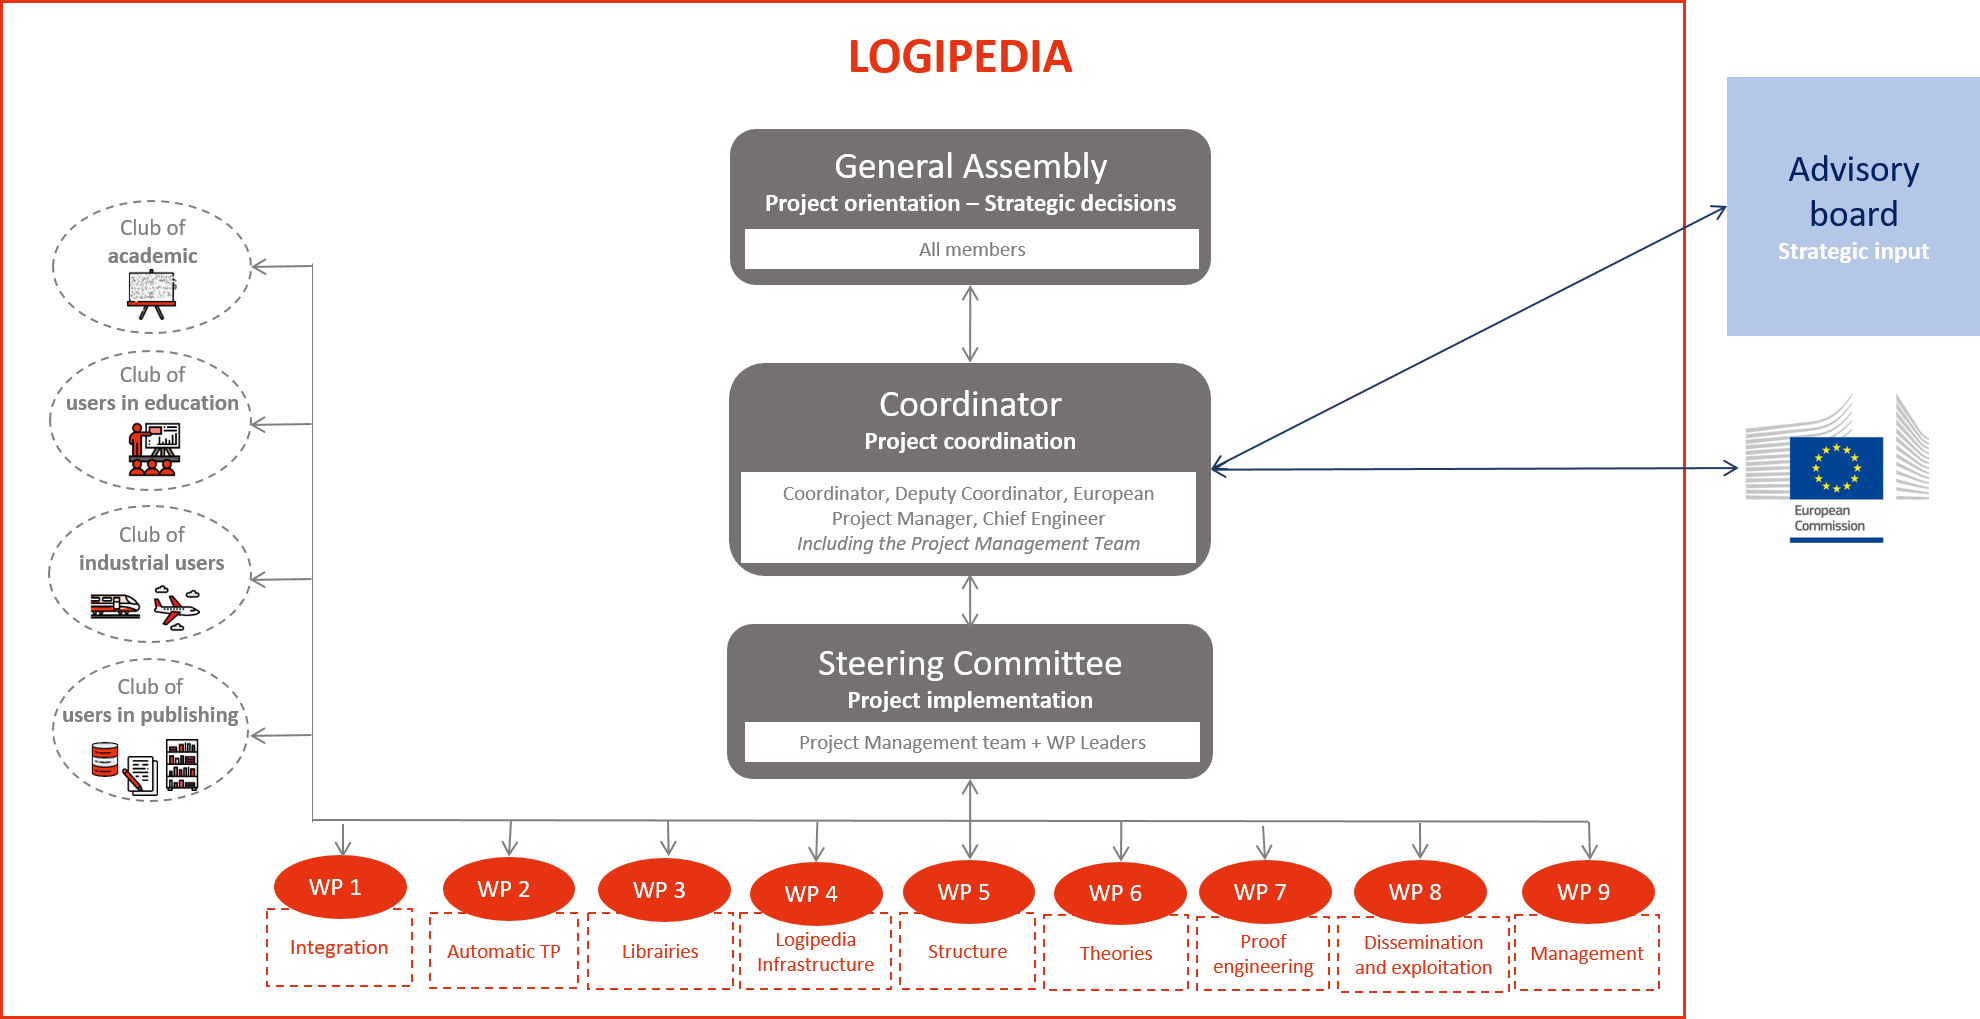
\includegraphics[width=\textwidth]{img/Gouvernance}

In this picture add the EC (talks to Coordinator only)

vice coordinator -> Deputy coordinator

Names of WP

Place of the cooddinator : outside of the bulbe talks to the SN

General assembly talks to SC (and not the SC is part of it)


\subsubsection*{The project management team}

\begin{compactitem}
\item{\bf The Coordinator}: the 
coordinator is responsible for the coordination of
scientific and technical activities in order to meet the objectives
set by the European Commission in the Grant Agreement. The 
coordinator works closely with the work package leaders
within the steering committee, in order to monitor the progress of the
scientific and technical work and identify potential risks within each
work package. The coordinator will daily
collaborate with the European project manager in charge of the
day-to-day management of Logipedia. The project will be managed by Pr
Gilles Dowek, permanent senior researcher at Inria Saclay. He will
also chair the meetings of both the general assembly and steering
committee.

\item{\bf The Deputy Coordinator}: The Deputy coordinator, Frédéric
Blanqui, seconds and replaces the coordinator if needed.

\item{\bf The European Project Manager}: The European project manager
  is a team member of the Technology Transfer and Partnership Office
  of Inria Saclay. He or she is in charge of all administrative,
  financial and legal management tasks as listed in
  \WPref{management}. The European project manager is the interface
  between the project and the European Commission as it represents the
  point of contact for the European Commission. The European project
  manager has the overall administrative and financial responsibility
  for the organisation and administrative and financial monitoring of
  the project.

\item{\bf The Chief Engineer}: The chief engineer is an experienced
research engineer from Inria Saclay and is responsible for ensuring
the development and maintenance of tools at Inria Saclay and
supervising the development tasks achieved at the other
beneficiaries. The chief engineer will ensure the coherence of the
Logipedia tools development, according to the defined schedule in the
Grant Agreement.
\end{compactitem}

Innovation management and intellectual property rights issues will be
handled by the European project manager, supported by the experienced
Technology Transfer and Partnerships Office of Inria Saclay. The
project management team will establish appropriate policies and rules
for the management of intellectual property rights for the knowledge
developed within the project, as well as the identification of the
opportunities for the exploitation of the project results in
innovation activities. Issues related to innovation and/or
intellectual property rights management will be tackled at every
steering committee meeting.

\subsubsection*{The operational level}

\begin{compactitem}
\item{\bf The Steering Committee}: The steering committee is composed
  of the Coordinator, the Deputy coordinator, the chief engineer, the
  European project manager and the work package leaders. The steering
  committee is the supervisory body for the implementation of the
  project. The steering committee is responsible innovation,
  intellectual property, and for monitoring the activities of the
  project and the implementation of decisions taken by the general
  assembly. It can formulate proposal for changes in the description
  of action and the related consortium budget. Those changes will have
  to be agreed by the general assembly first and then the European
  commission. The steering committee is chaired by the coordinator.

\item{\bf The Work Package Leaders}: The work package leaders are
responsible for the monitoring and management of the activities and
results within their work packages. In particular, work package
leaders i) identify deviations from the project plan and report them
to the steering committee, ii) manage and supervise the preparation of
reports and their timely delivery, iii) control and monitor activities
of tasks and regularly meet once per month with task leaders, iv)
manage the information flow with other work packages via the steering
committee.

\item{\bf The Task Leaders}: The task leaders are responsible for
coordinating the scientific and technical work in their task and
making the day to day technical decisions that solely affect their
task. Inter-task decisions are coordinated with the work package
leaders.

\item{\bf The Club Leaders}: The club leaders are in charge of
disseminating of the tools developed by the Logipedia consortium in
various communities. They organize the activity of the club. They give
ongoing feedback to the consortium during the course of the project.
\end{compactitem}

\subsubsection*{The strategic level}

\begin{compactitem}
\item{\bf The General Assembly}: The general assembly is composed by all
the members of the consortium, with each representative having one
vote. Every new partner will have a voting right. The general assembly
will gather at least once a year, and as many virtual meetings as
needed. The general assembly is the main governance and ultimate
decision-making body of the consortium. The general assembly must
review the project progress, decide on contingency actions in case of
deviations from the plan and take final decisions on policy and
contractual issues and conflicts as requested by the steering
committee.

\item{\bf The Advisory Board}: The advisory board is a consultation body to
the steering committee and general assembly. It will bring external
and non-legally binding perspective on the scientific and technical
development of the project, ecosystem building and the future of the
encyclopedia. The advisors of this board will attend the yearly
general assembly plenary meeting and will be consulted on the strategy
of the project. The advisory board should aim at representing the
stakeholders of the Logipedia ecosystem without including any
beneficiary or associate partner’s employees. It will be composed of,
among others, industrial and international academic partners
(including non-European ones) apointed by the coordinator after
consulting the steering committee. To start with, we suggest to
include: June Andronick (Data61, Kensington NSW, AU), Denis Cousineau
(Mitsubishi Electric R\&D Centre Europe, FR), Thomas Letan (ANSSI, FR),
Jacques Fleuriot (University of Edinburgh, UK), Natarajan Shankar
(SRI, US), Aaron Stump (Iowa University, US), Laurent Voisin
(Systerel, FR).
\end{compactitem}

\subsubsection*{Internal communication and collaborative ecosystem}

The communication of the consortium including their internal tools is
managed in task 10.2.  The consortium will make use of a number of
project management tools, such as a visio conferencing tool, a project
repository to have an updated account of the project’s important
documents, the progress of the work packages work and deliverables,
all the advances in the project and all the meetings minutes, mailing
lists, etc. that facilitate the smooth execution of the project. This
collaboration environment will be provided by the coordinator of the
project.

Work packages, chaired by work package leaders, will have monthly
planned visio conferences and meetings as need by the work plan;
additional technical meetings may be set up by task leaders or
individual partners. The steering committee will have monthly visio
conferences and will meet twice a year. Dedicated working groups will
be planned as needed according to the work plan.  All meetings will be
documented by minutes listing major decisions and action items.

The project management team will be in charge of all organisational
issues in the general assembly meetings, supported by the local
partner. The project will organise meetings of the general assembly at
least once a year. To equally share travel costs among partners,
physical meetings will be located by rotation at partners’
locations. Project review meetings will be done on a regular basis
according the Grant Agreement provisions.

%%%%%%%%%%%%%%%%%%%%%%%%%%%%%%%%%%%%%%%%%%%%%%%%%%%%%%%%%%%%%%%%%%%%%%%%%%%%%%
\subsection{Decision-making Process}

Our approach for the decision-making process is to locate the decision
as close as possible to the level responsible for the execution (from
task to general assembly level). Decisions are managed within
frequent project meetings, either on-site or via
teleconference. Decisions can be also managed by consultation. If
voting is needed, the agenda should clearly indicate this fact. Quorum
and voting rules will be defined in the Consortium
Agreement. Decisions are binding once the relevant part of the meeting
minutes has been accepted. Any changes to the project plan and scope
must be reviewed and approved by all levels of project management,
before proposing these changes to the steering committee and any
modifications will be considered rejected, after rejection on any of
these involved levels.

Another guiding principle is to avoid conflicts. Nevertheless, should
one arise, a conflict resolution will be ready to be put in place to
deal with it accordingly. The conflict resolution foresees that each
conflict will be mediated, solved or decided at the lowest level
possible. Attempts to solve issues within the consortium will be
carried out in increasing order of authority first at task level
(management of task leader), work package level (management of work
package leaders), and then following the management bodies till the
general assembly. Further rules related to conflict resolutions will
be laid out in the Consortium Agreement.

%%%%%%%%%%%%%%%%%%%%%%%%%%%%%%%%%%%%%%%%%%%%%%%%%%%%%%%%%%%%%%%%%%%%%%%%%%%%%%
\subsection{Monitoring and reporting}

\subsubsection*{Internal reporting}

The project management team continuously monitors the project plan
with its milestones. Each work package leader will be
responsible for the correct execution of the implementation plan for
the corresponding work package. In terms of reporting, this means the work package leaders
will be in charge of gathering the information related to their own
work packages.

Regular audio-conferences of the Steering Committee are foreseen,
which allows work package leaders to identify risks and
discuss them together. This ensures that management (coordination,
European project manager) is aware of potential problems and
deviations and can initiate countermeasures long before a situation
becomes critical. This ensure to spot the blocking points and implements
the solution at the right time.


In case there is a deviation from the work plan, the 
coordinator will initiate corrective actions through the
task leader and the work package leader. The work package leader will
be responsible to implement these actions in dialogue with the
different partners involved in their work packages.

\subsubsection*{Reporting to the European Commission}

The Logipedia consortium will follow the mandatory reporting period
required by the European Commission. 

The project management team will provide the necessary templates in
order to achieve the reporting in due time. Work package leaders will
be asked to gather the relevant information provided by the task
leader regarding their work package and to summarise in order to be
reviewed by the steering committee. It will then be treated by the
coordinator and European project manager and sent to the
European Commission.

%%%%%%%%%%%%%%%%%%%%%%%%%%%%%%%%%%%%%%%%%%%%%%%%%%%%%%%%%%%%%%%%%%%%%%%%%%%%%%
\subsection{Significant risks and associated contingency plans}
\label{sec:risks}

\subsubsection*{Scientific risks}

\begin{longtable}{|p{0.30\textwidth}|p{0.10\textwidth}|p{0.50\textwidth}|}
\hline
{\bf Description of the risk}
&
{\bf Work packages involved}
&
{\bf Proposed measure of mitigation}
\\
\hline
Some theories are difficult to express in Dedukti.
(Probability: medium. Severity: low.)

{\color{red} It is not that it is difficult that is a risk, it is
that we fail to do it}
&
WP6
&
We have carefully divided the systems into two groups: those that do not
present risks (WP1) and those that do (WP6). The success we got with the
theories implemented in systems of the first group gives us confidence
that the theories implemented in those of the second can also be
expressed in Dedukti.  If one of them happens to be more difficult, we
can still build a large encyclopedia with the systems of the first
group. We can also extend Dedukti so that it can express more theories,
as we have already done in the past.
\\
\hline
Some libraries require too much time and memory
to be expressed in Dedukti (Probability: medium. Severity: low.)
&
WP3
&
There are several ways to mitigate this risk: optimize the
representation of data (sharing, elimination of redundancies, etc.), 
use faster and larger computers. This may also mean that some tasks
of this work package are premature and that we have to wait for
faster computers, that Moore's law will provide.
\\
\hline
No adoption from the community. (Probability: low. Severity: high.)
&
All 
&
The community may fail to adopt Logipedia for several reasons. Because
of a problem of design of Logipedia, in which case we will have to
understand what needs to be changed in a second version.  It may be
because the Logipedia community is too small.  This explains that we
have decided to include twenty-eight partners in the project.  It may
also be because of an insufficient dissemination activity.  This is
why we propose to create the four clubs of users and we will devote
time and energy to the animation of these clubs, together with other
dissemination activities, such as summer schools and conferences.
\\
\hline
\end{longtable}

\subsubsection*{Management risks}

\begin{longtable}{|p{0.30\textwidth}|p{0.10\textwidth}|p{0.50\textwidth}|}
\hline
Brexit disrupts the project (Probability: low. Severity: medium.)
&
All (specially WP6, WP7)
&
As we have two partners from the United Kingdom, Brexit could be a risk
for our project. Yet, we are quite confident
that scientific
cooperation will continue after Brexit and that the British partners
of the project will continue to be part of it.
As this project is submitted during H2020 and nothing changes until
the end of 2020, Logipedia is safe for the start of the project. From
2021 onwards, we can hope some agreement will be concluded as the UK
already made public its willingness to maintain collaborations.
If it were not the
case, we would have to reallocate the impacted tasks to other partners. 
\\
\hline
One partner leaves (Probability: low. Severity: depends on the partner.)
&
All
&
The impact of such a default of one partner of course depends on the
partner. But, during the preparation of this project, we have been
careful to develop an atmosphere of trust and solidarity between the
partners. If this happened
we would need to adapt the objectives of the work package the partner
was supposed to contribute to.
\\
\hline
Difficulty to find people (doctoral students, post-docs, engineers, etc.)
(Probability: medium. Severity: low.)
&
All
&
This project will require hiring a fair number of people. This may be
difficult in some European countries. If this happens we will use the
size of the network to find candidates in other countries to meet
the objectives of the project.\\
\hline
\end{longtable}

%%%%%%%%%%%%%%%%%%%%%%%%%%%%%%%%%%%%%%%%%%%%%%%%%%%%%%%%%%%%%%%%%%%%%%%%%%%%%%
\subsection{Milestones}\label{sec:milestones}

{\color{red} Bad idea, to have all milestones < 24}


As show by the Pert diagram above, two work packages, are critical, as
many others depend on them: work package 4 ``Access to the
encyclopedia'' that is focused on the development of the
infrastructure itself and work package 1 ``Integration'' that focuses
on populating this infrastructure with theories and proofs. All work
packages depend on work package 4, and work packages 3 ``Large
libraries'', work package 5 ``Structure of the encyclopedia'', and
work package 7 ``Proof engineering'' depend on work package 1.
As a consequence our milestones are completions of the key tasks of
work packages 4 and 1.

All milestones have to be completed in the first and second year
of the project, which is a sign of controllability of the project.
No milestone is the completion of a
task of the two, more risky, joint research activity work packages:
work package 6 ``Theories'' and work package 7 ``Proof engineering'',
which is a sign of robustness of the project.
  

%\begin{longtable}{|p{0.1\textwidth}|p{0.55\textwidth}|p{0.2\textwidth}|p{0.1\textwidth}|}
%%%%%%%%%%%%%%%%%%%%%%%%%%%%%%%%%%%%%%%%%%%%%%%%%%%%%%%%%%%%%%%%%%%%%%%%%%%%%%
%\hline
%1
%&
%Prototype version of Logipedia platform
%&
%deliverable D4.7
%&
%M 14
%\\
%\hline
%2
%&
%Opam for Logipedia
%&
%deliverable D4.3
%&
%M 20
%\\
%\hline
%\end{longtable}

%\begin{longtable}{|p{0.1\textwidth}|p{0.55\textwidth}|p{0.2\textwidth}|p{0.1\textwidth}|}
%%%%%%%%%%%%%%%%%%%%%%%%%%%%%%%%%%%%%%%%%%%%%%%%%%%%%%%%%%%%%%%%%%%%%%%%%%%%%%
%\hline
%3
%&
%Instrumentation of Isabelle 
%&
%deliverable D1.2
%&
%M 12
%\\
%\hline
%4
%&
%Instrumentation of HOL4 
%&
%deliverable D1.3
%&
%M 12
%\\
%\hline
%5
%&
%Instrumentation of Coq 
%&
%deliverable D1.6
%&
%M 8
%\\
%\hline
%\end{longtable}

{\color{red} order the milestones by date}

  
\begin{milestones}
\milestone[id=platform,verif=Inspection,month=14]
  {Prototype version of the Logipedia platform}
  {Release of a first version of the Logipedia platform}
\milestone[id=opam,verif=Inspection,month=20]
   {Opam for Logipedia}
   {Release of a first version of Opam for Logipedia}
\milestone[id=isabelle,verif=Inspection,month=12]
   {Instrumentation of Isabelle}
   {Integration of the Isabelle standard library in Logipedia}
\milestone[id=hol4,verif=Inspection,month=12]
   {Instrumentation of HOL4}
   {Integration of the HOL4 standard library in Logipedia}
\milestone[id=coq,verif=Inspection,month=8]
   {Instrumentation of Coq}
   {Integration of the Coq standard library in Logipedia}
\end{milestones}

{\


%%% Local Variables:
%%%   mode: latex
%%%   mode: flyspell
%%%   ispell-local-dictionary: "english"
%%% End:


\section{Consortium as a whole}\label{sec:consortium}

\begin{todo}{}\color{red}
  The individual members of the consortium are described in a separate section 4. There is no need to repeat that information here.

  Describe the consortium. How will it match the project’s objectives, and bring together the necessary expertise? How do the members complement one another (and cover the value chain, where appropriate)? 

  In what way does each of them contribute to the project? Show that each has a valid role, and adequate resources in the project to fulfil that role. 

  If applicable, describe the industrial/commercial involvement in the project to ensure exploitation of the results and explain why this is consistent with and will help to achieve the specific measures which are proposed for exploitation of the results of the project (see section 2.2). 

  Other countries and international organisations: If one or more of the participants requesting EU funding is based in a country or is an international organisation that is not automatically eligible for such funding (entities from Member States of the EU, from Associated Countries, from one of the countries in the exhaustive list included in General Annex A of the work programme, and, under specific conditions, from further countries identified in the work programme1,are automatically eligible for EU funding), explain why the participation of the entity in question is essential to carrying out the project .
\end{todo}

\begin{todo}{from the proposal template}
  Describe how the participants collectively constitute a consortium capable of achieving
  the project objectives, and how they are suited and are committed to the tasks assigned
  to them. Show the complementarity between participants. Explain how the composition of
  the consortium is well-balanced in relation to the objectives of the project.  

  If appropriate describe the industrial/commercial involvement to ensure exploitation of
  the results. Show how the opportunity of involving SMEs has been addressed
\end{todo}

The project partners of the \pn project have a long history of successful collaboration;
Figure~\ref{tab:collaboration} gives an overview over joint projects (including proposals) and
joint publications (only international, peer reviewed ones).

\jointorga{Fau,Bol}% CICM
\jointorga{Inn,Bol}% CICM
\jointpub{Fau,Bol}% CICM paper
\jointpub{Tum,Bol}% CICM paper
\jointpub{Fau,TUM}% 
%\jointsup{Fau,}
\jointsoft{Fau,Tum}% Isabelle Extension
\jointsoft{Fau,Bol}% Coq exporter
\jointpub{Inr,Bol}% ELPI
\jointproj{Inr,Bol}% MoWGLI
\coherencetable

\subsection{Subcontracting}\label{sec:subcontracting}
\begin{todo}{from the proposal template}
  If any part of the work is to be sub-contracted by the participant responsible for it,
  describe the work involved and explain why a sub-contract approach has been chosen for
  it.
\end{todo}

\ednote{@Rabe: justify subcontracting for Wenzel}

\subsection{Other Countries}\label{sec:other-countries}
\begin{todo}{from the proposal template}
  If a one or more of the participants requesting EU funding is based outside of the EU
  Member states, Associated countries and the list of International Cooperation Partner
  Countries\footnote{See CORDIS web-site, and annex 1 of the work programme.}, explain in
  terms of the project’s objectives why such funding would be essential.
\end{todo}

\subsection{Additional Partners}\label{sec:assoc-partner}
\begin{todo}{from the proposal template}
  If there are as-yet-unidentified participants in the project, the expected competences,
  the role of the potential participants and their integration into the running project
  should be described
\end{todo}

%%% Local Variables:
%%% mode: latex
%%% TeX-master: "propB"
%%% End:


\section{Resources to be Committed}\label{sec:resources}

\begin{todo}{}\color{red}
Please make sure the information in this section matches the costs as stated in the budget table in section 3 of the administrative proposal forms, and the number of person months, shown in the detailed work package descriptions.

Please provide the following:

- a table showing number of person months required (table 3.4a)

- a table showing ‘other direct costs’ (table 3.4b) for participants where those  costs exceed 15\% of the personnel costs (according to the budget  table in section 3 of the administrative proposal forms) and participants providing trans-national access under this project and incurring travels and subsistence costs for supporting users' access.

Please note that the distribution of resources between access (TA/VA), JRA, and NA components must be duly justified.
\end{todo}

\subsection{Travel Costs and Consumables}\label{sec:travel-costs}
\subsection{Subcontracting Costs}

\ednote{@Rabe: add subcontracting cost for Wenzel for WP 7}

\subsection{Other Costs}

%%% Local Variables: 
%%% mode: LaTeX
%%% TeX-master: "propB"
%%% mode: flyspell
%%% ispell-local-dictionary: "english"
%%% End: 

% LocalWords:  pn newpage site-FAU site-efo site-baz jointpub efo baz
% LocalWords:  jointproj coherencetable assoc-partner
